\chapter{Conception et Mise en place}

\section*{Introduction}

Le chapitre précédent a établi les choix technologiques retenus pour chaque module :
l'architecture RAG avec ChromaDB et Mistral-7B pour les modules conversationnels,
le LLM conversationnel avec profil persistant pour le soutien émotionnel,
et l'ancrage juridique combiné aux règles heuristiques pour le classificateur.
Ce chapitre couvre deux phases étroitement liées : la conception du système et la mise en place des modèles d'intelligence artificielle.
La première partie présente l'architecture commune aux quatre modules et la conception spécifique de chacun d'eux, illustrée par des diagrammes UML (Unified Modeling Language — langage de modélisation unifié).
La seconde partie décrit la préparation des données et la construction des bases de connaissances pour les modules RAG, ainsi que le cycle complet d'apprentissage du classificateur de harcèlement.

% ─────────────────────────────────────────────────────────────────────────────
\section{Architecture commune du système}

\subsection{Vue d'ensemble}

Les quatre modules du système partagent des composants technologiques communs.
Cette conception modulaire facilite la maintenance et l'évolution du système.
La Figure~\ref{fig:composants_global} illustre l'architecture globale.

\begin{figure}[H]
\centering
\hspace*{-0.1\textwidth}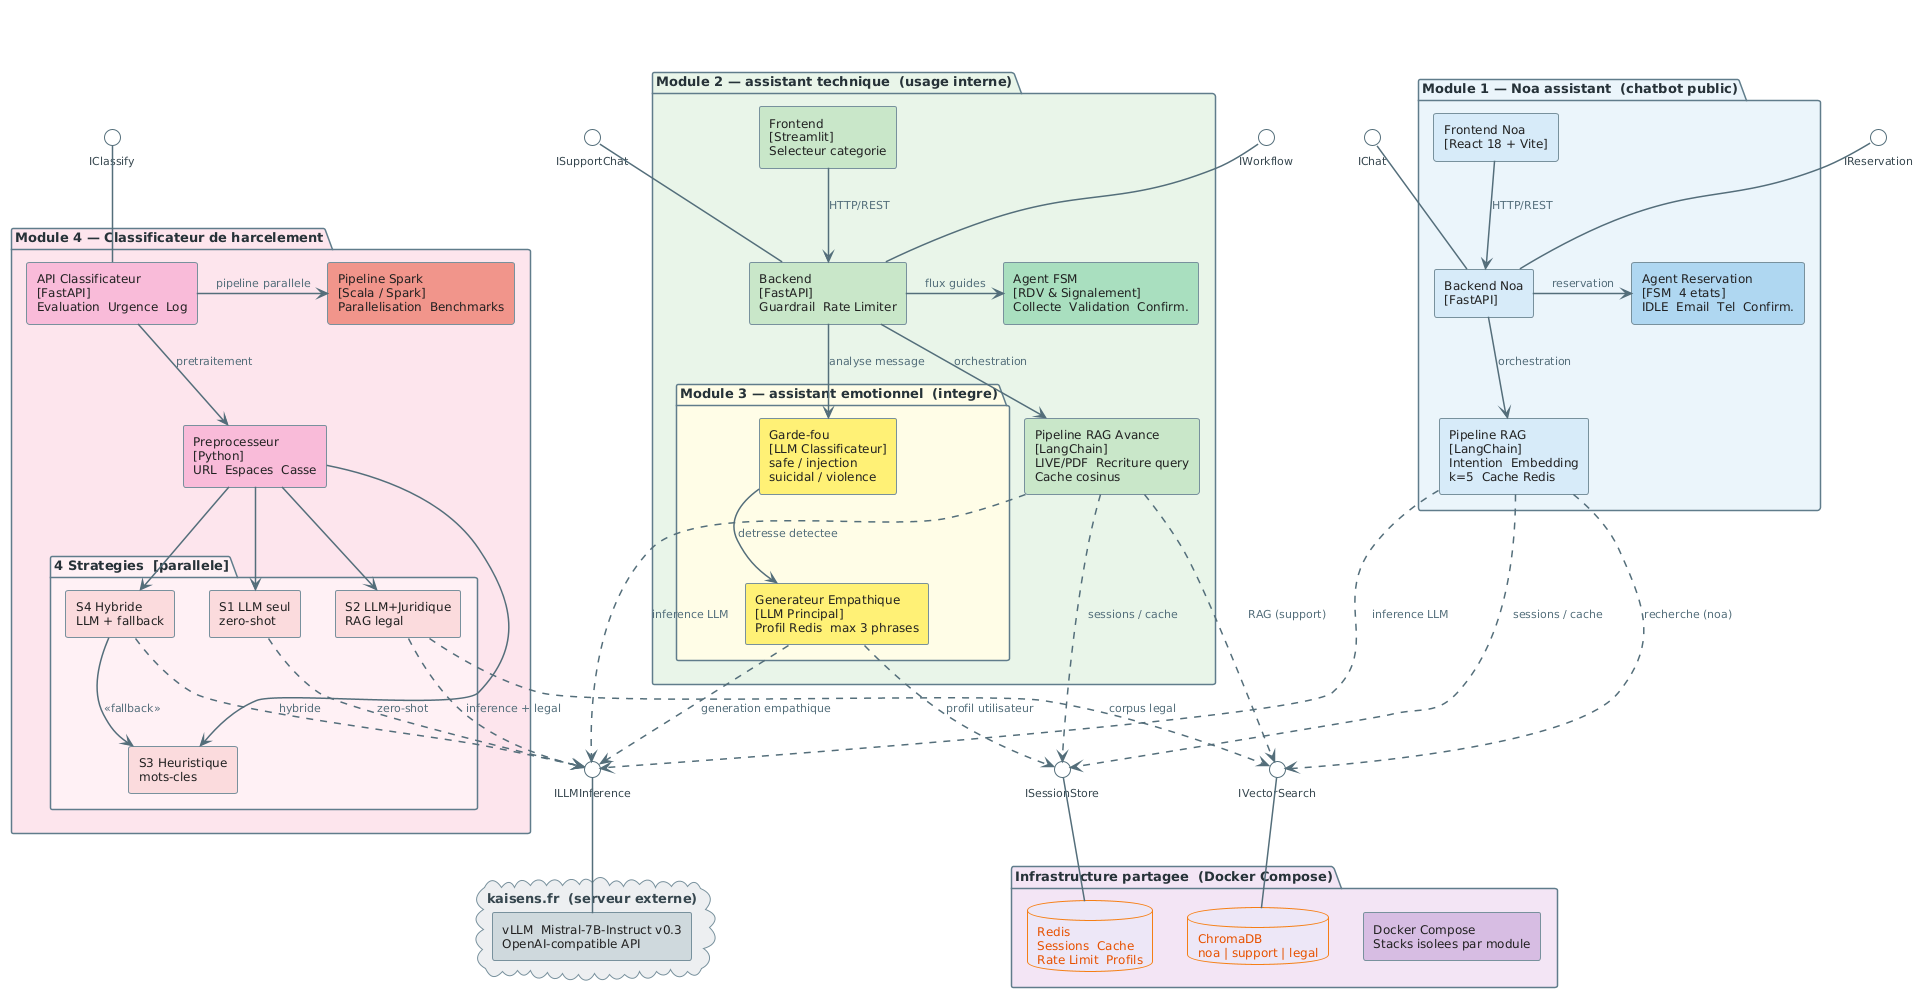
\includegraphics[width=1.2\textwidth]{diagramme/12_composants_architecture.png}
\caption{Diagramme de composants — Architecture globale du système}
\label{fig:composants_global}
\end{figure}

\subsection{Composants partagés}

Les composants suivants sont utilisés par plusieurs modules :

\begin{itemize}
    \item \textbf{Serveur LLM partagé (kaisens.fr) :} Point central de génération de réponses
          en langage naturel pour les quatre modules.
          Il s'appuie sur vLLM avec le modèle Mistral-7B-Instruct v0.3 sur GPU NVIDIA A100,
          exposé via une interface compatible OpenAI (\texttt{POST /v1/chat/completions}).
    \item \textbf{Base documentaire vectorielle (ChromaDB) :} Stocke les extraits de documents
          indexés pour la recherche par similarité sémantique.
          Chaque module possède sa propre collection : l'assistant Noa et l'assistant technique
          embarquent ChromaDB directement dans leur conteneur API,
          tandis que le Classificateur l'instancie comme service Docker dédié.
    \item \textbf{Gestionnaire de mémoire (Redis) :} Assure la persistance des sessions
          conversationnelles, le cache sémantique cosinus et la limitation de débit \cite{redis}.
    \item \textbf{Orchestrateur LangChain :} Coordonne les étapes de traitement
          pour les modules conversationnels (Noa, Support, Soutien émotionnel) :
          classification d'intention, recherche documentaire, appel LLM
          et gestion de session \cite{langchain}.
    \item \textbf{Conteneurisation Docker :} Chaque module est déployé dans sa propre stack
          Docker Compose isolée, garantissant la reproductibilité, la portabilité
          et l'indépendance entre modules \cite{docker}.
\end{itemize}

\subsection{Architecture de déploiement}

Chaque module est déployé de manière indépendante dans sa propre stack Docker Compose.
Cette isolation garantit qu'un module peut être mis à jour, redémarré ou remplacé
sans affecter les autres.
La Figure~\ref{fig:deploiement} présente la vue d'ensemble du déploiement avec les quatre stacks et le LLM partagé.
Les diagrammes de déploiement détaillés de chaque module sont fournis dans les sections correspondantes.

\begin{figure}[H]
\centering
\hspace*{-0.1\textwidth}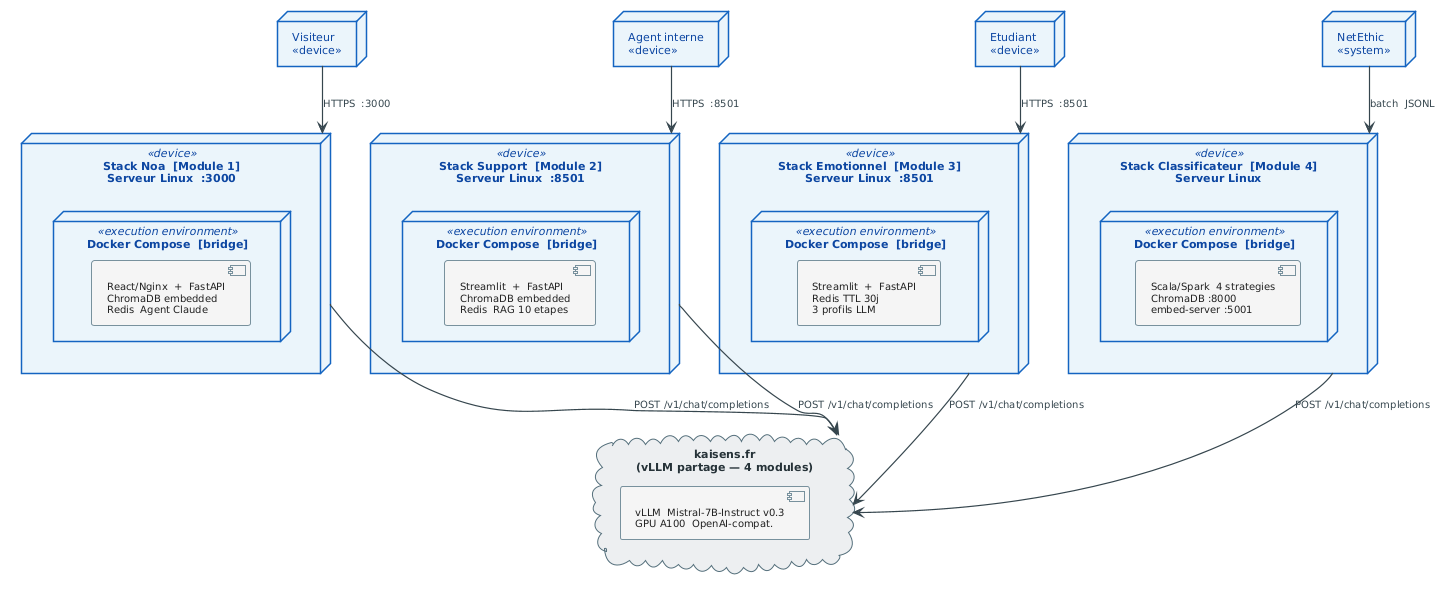
\includegraphics[width=1.2\textwidth]{diagramme/13_deploiement_uml.png}
\caption{Vue d'ensemble du déploiement — 4 stacks indépendantes de la plateforme NetEthic AI}
\label{fig:deploiement}
\end{figure}

% ─────────────────────────────────────────────────────────────────────────────
\section{Module 1 — Assistant Noa}

\subsection{Conception générale}

Noa est l'assistant virtuel accessible sur le site public de Netethic.
Son architecture repose sur un pipeline à cinq étapes :
classification de l'intention, vérification du cache, recherche documentaire,
génération de la réponse et mise à jour du cache.

\textbf{Routage par intention.}
Chaque message est classifié avant tout traitement.
Les salutations et demandes hors sujet reçoivent des réponses prédéfinies immédiates,
court-circuitant le pipeline RAG complet.

\textbf{Stratégie parent-enfant.}
Les documents sont indexés à deux niveaux : les segments courts (enfants) servent
à la recherche par similarité sémantique, tandis que les segments longs (parents)
sont transmis au LLM pour générer une réponse contextuellement riche.

\textbf{Normalisation des questions fréquentes.}
Deux questions au sens identique partagent la même réponse mémorisée,
grâce à une normalisation par synonymes avant la consultation du cache Redis.

\textbf{Agent de réservation.}
Un automate à états finis guide l'utilisateur lors de la collecte de son adresse
e-mail et de son numéro de téléphone pour planifier une démonstration.

\subsection{Diagramme de composants}

La Figure~\ref{fig:composants_noa} illustre l'organisation interne du module Noa en trois couches (présentation, métier et données) ainsi que les interactions entre ses composants principaux.

\begin{figure}[H]
\centering
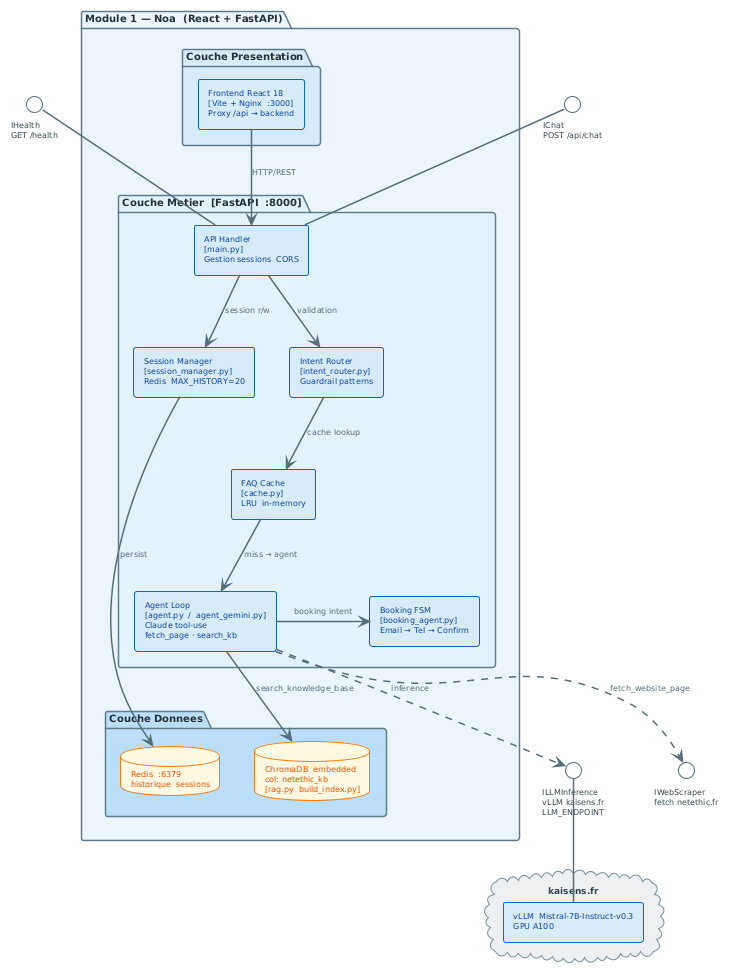
\includegraphics[width=\textwidth]{diagramme/18_composants_noa.png}
\caption{Diagramme de composants — Assistant Noa}
\label{fig:composants_noa}
\end{figure}

\subsection{Diagramme de déploiement}

La Figure~\ref{fig:deploiement_noa} présente la stack Docker Compose du module Noa avec ses conteneurs et leurs interconnexions.

\begin{figure}[H]
\centering
\hspace*{-0.1\textwidth}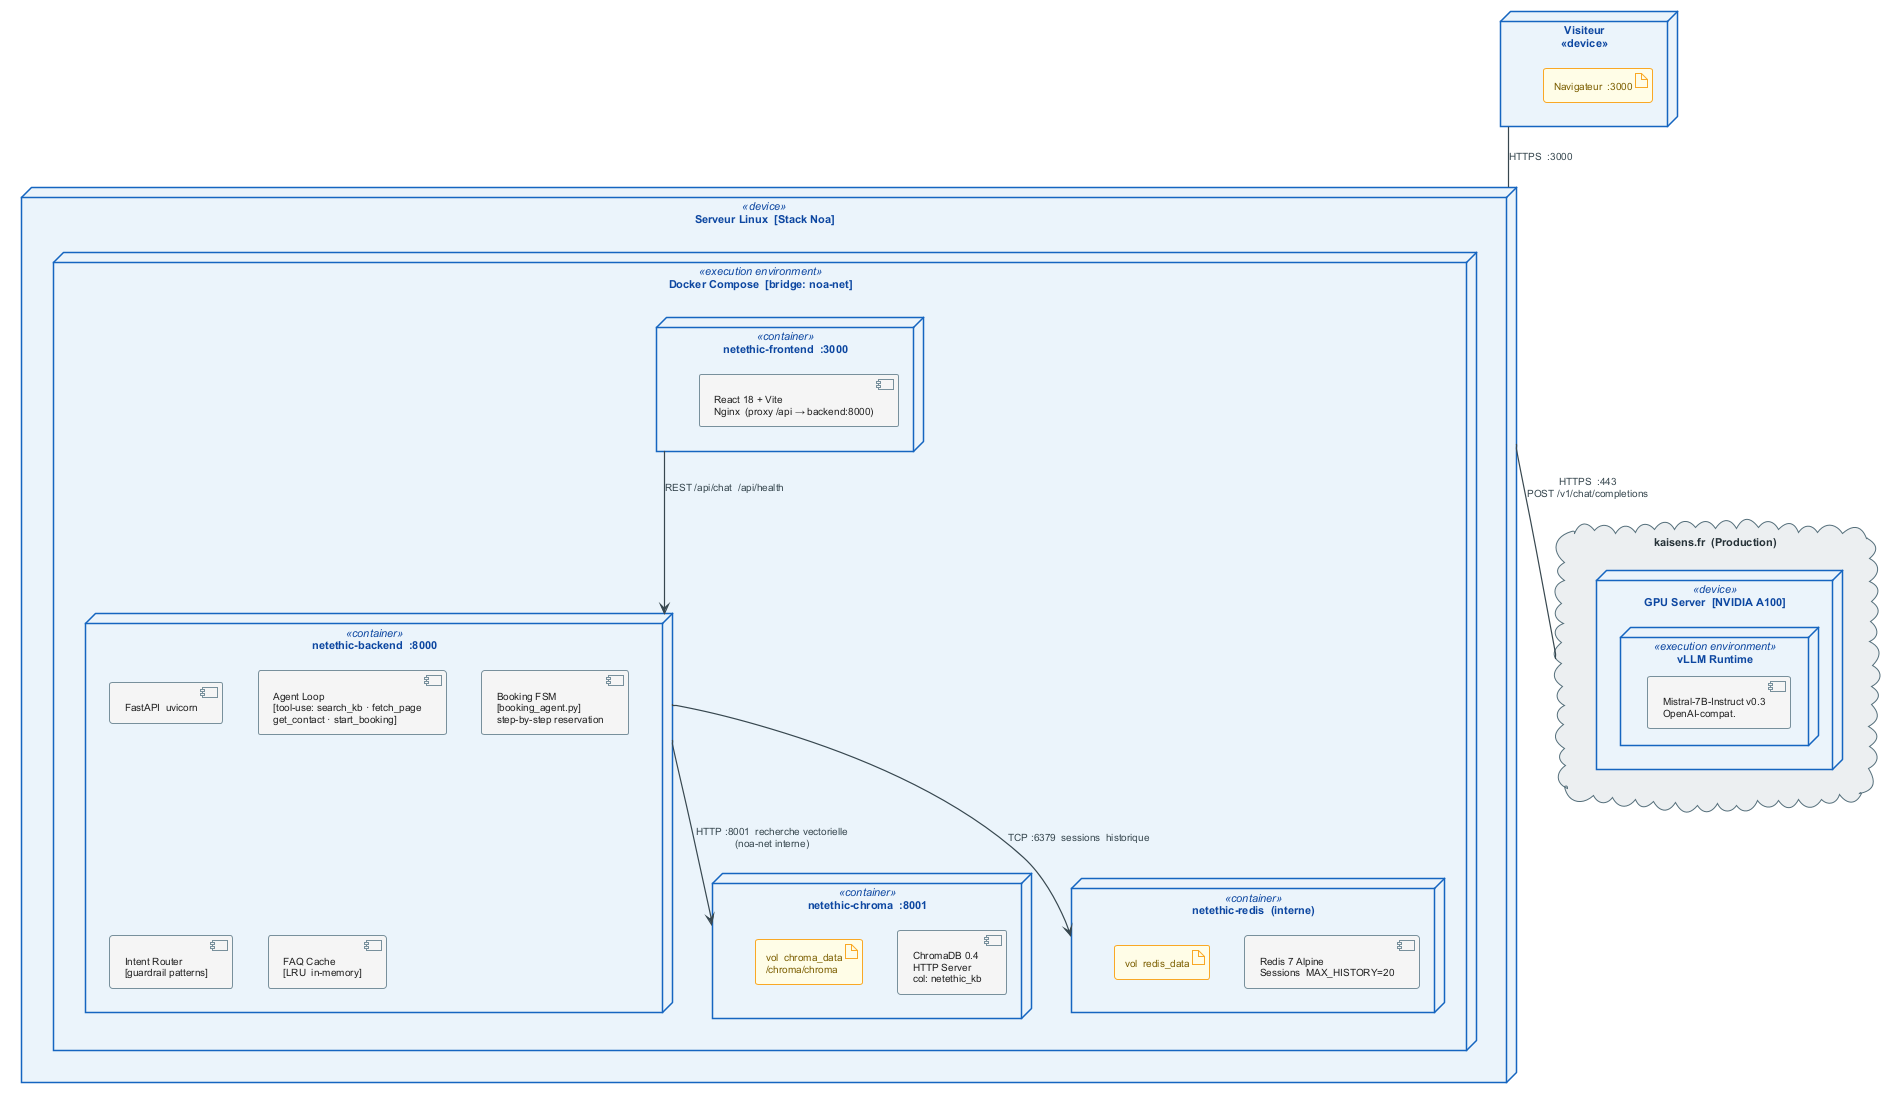
\includegraphics[width=1.2\textwidth]{diagramme/14_deploiement_noa.png}
\caption{Diagramme de déploiement — Assistant Noa (stack Docker Compose)}
\label{fig:deploiement_noa}
\end{figure}

\subsection{Diagramme de séquences}

La Figure~\ref{fig:seq_noa} illustre le déroulement d'une interaction typique avec Noa
pour une question factuelle.

\begin{figure}[H]
\centering
\hspace*{-0.1\textwidth}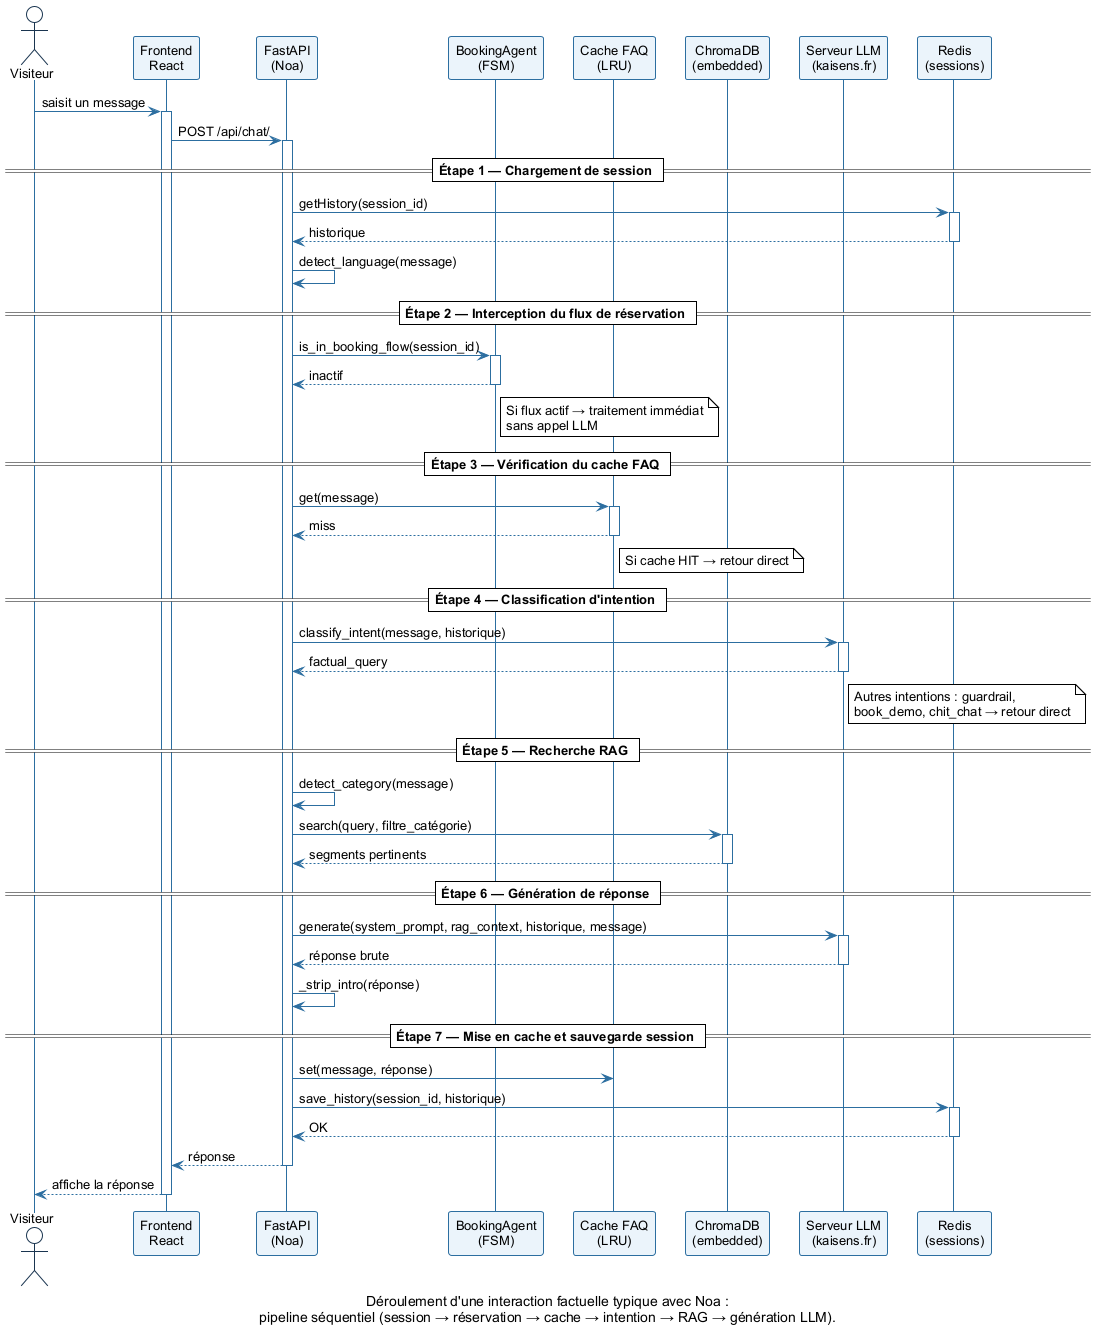
\includegraphics[width=1.2\textwidth]{diagramme/04_sequence_noa.png}
\caption{Diagramme de séquences — Assistant Noa (question factuelle)}
\label{fig:seq_noa}
\end{figure}


% ─────────────────────────────────────────────────────────────────────────────
\section{Module 2 — Assistant technique}

\subsection{Conception générale}

L'\textit{assistant technique} est l'assistant de support technique
destiné aux utilisateurs internes de la plateforme.
Son pipeline repose sur les mêmes composants partagés que l'assistant Noa
(serveur LLM, ChromaDB, Redis, LangChain),
mais introduit deux mécanismes architecturaux distincts.

\textbf{Double pipeline LIVE/PDF.}
À l'ouverture de session, la plateforme injecte un instantané JSON du tableau de bord
directement dans la session utilisateur.
Un classificateur d'intention LLM sépare ensuite les questions portant sur des métriques
en temps réel (\textit{LIVE}) des questions documentaires (\textit{PDF}).
Les premières sont traitées à partir des données de session uniquement,
sans appel à ChromaDB ; les secondes suivent le pipeline RAG standard.

\textbf{Flux de repli guidés.}
Lorsqu'aucun document pertinent n'est trouvé, le frontend déclenche trois flux
conversationnels à états finis : prise de rendez-vous, signalement de dysfonctionnement
(avec description auto-générée à partir de l'historique) et accès au portail de support.
Les informations d'identité de l'utilisateur, déjà présentes en session, pré-remplissent
les formulaires sans ressaisie.

L'interface est développée en Streamlit pour un déploiement rapide côté interne.

\subsection{Diagramme de composants}

La Figure~\ref{fig:composants_support} illustre l'architecture interne de l'assistant technique et les interactions entre ses composants.

\begin{figure}[H]
\centering
\hspace*{-0.1\textwidth}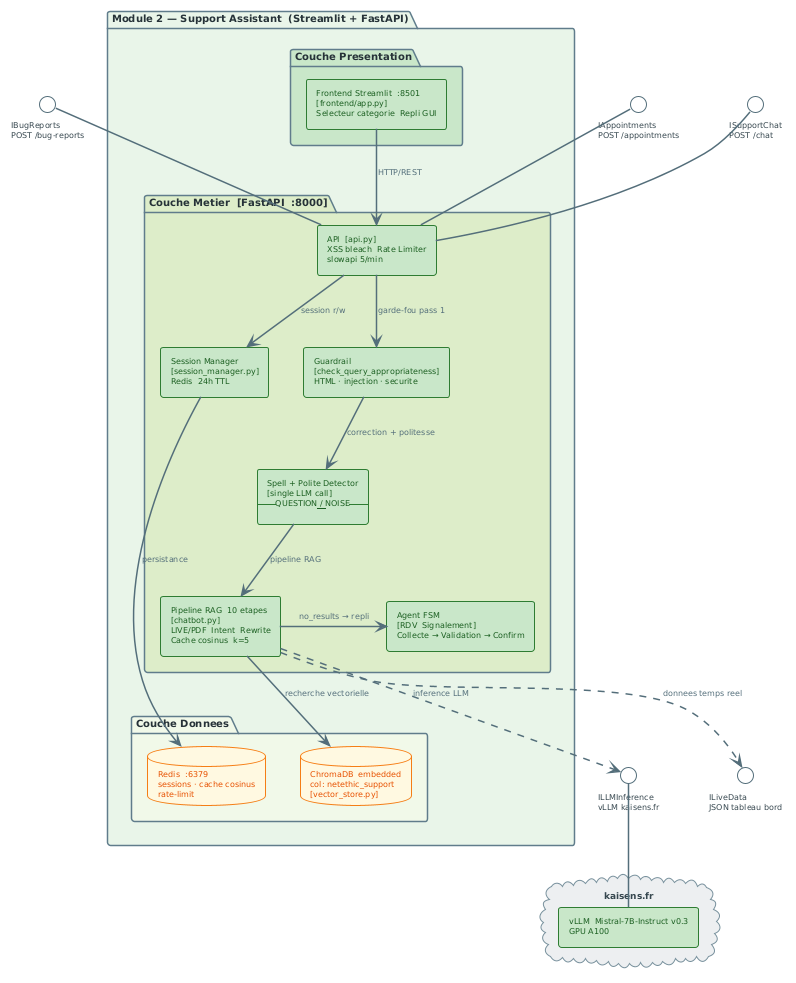
\includegraphics[width=1.2\textwidth]{diagramme/19_composants_support.png}
\caption{Diagramme de composants — Assistant technique}
\label{fig:composants_support}
\end{figure}

\subsection{Diagramme de déploiement}

La Figure~\ref{fig:deploiement_support} présente la stack Docker Compose de l'assistant technique avec ses conteneurs et leurs interconnexions.

\begin{figure}[H]
\centering
\hspace*{-0.1\textwidth}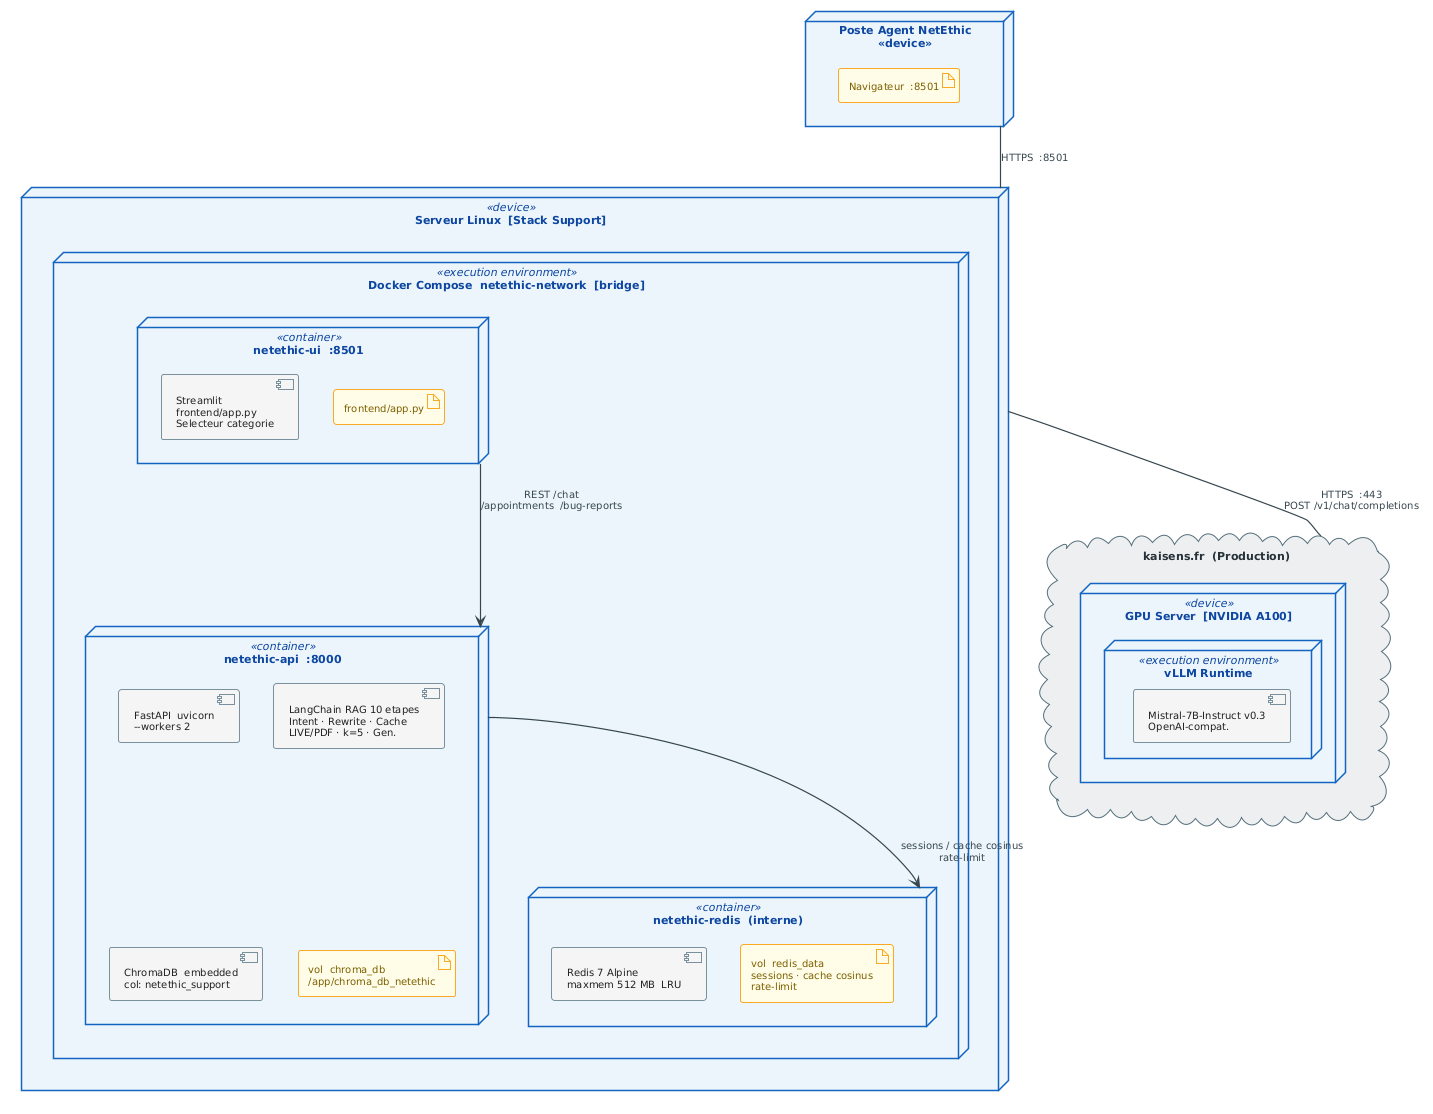
\includegraphics[width=1.2\textwidth]{diagramme/15_deploiement_support.png}
\caption{Diagramme de déploiement — Assistant technique (stack Docker Compose)}
\label{fig:deploiement_support}
\end{figure}

\subsection{Diagrammes de séquences}

Le traitement d'une question par l'assistant technique est décrit en trois parties.
La Figure~\ref{fig:seq_support_init} couvre la phase d'initialisation et de validation (étapes 1 à 10).

\begin{figure}[H]
\centering
\hspace*{-0.1\textwidth}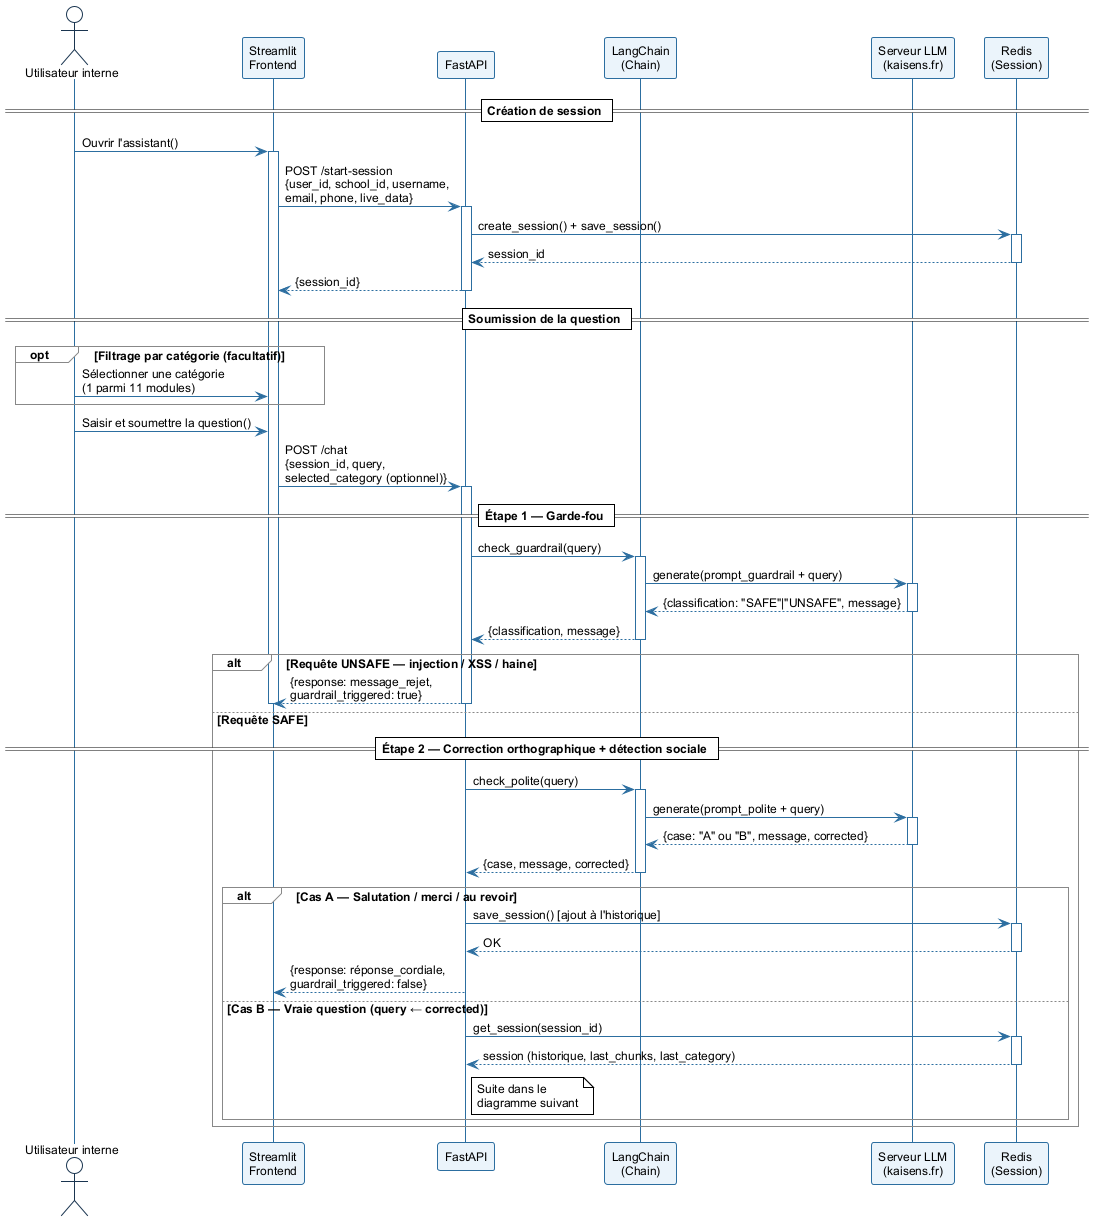
\includegraphics[width=1.15\textwidth]{diagramme/06a_sequence_support_init.png}
\caption{Diagramme de séquences — Assistant technique (1/3) : session et validation}
\label{fig:seq_support_init}
\end{figure}

La Figure~\ref{fig:seq_support} détaille le pipeline RAG (étapes 11 à 20).

\begin{figure}[H]
\centering
\hspace*{-0.1\textwidth}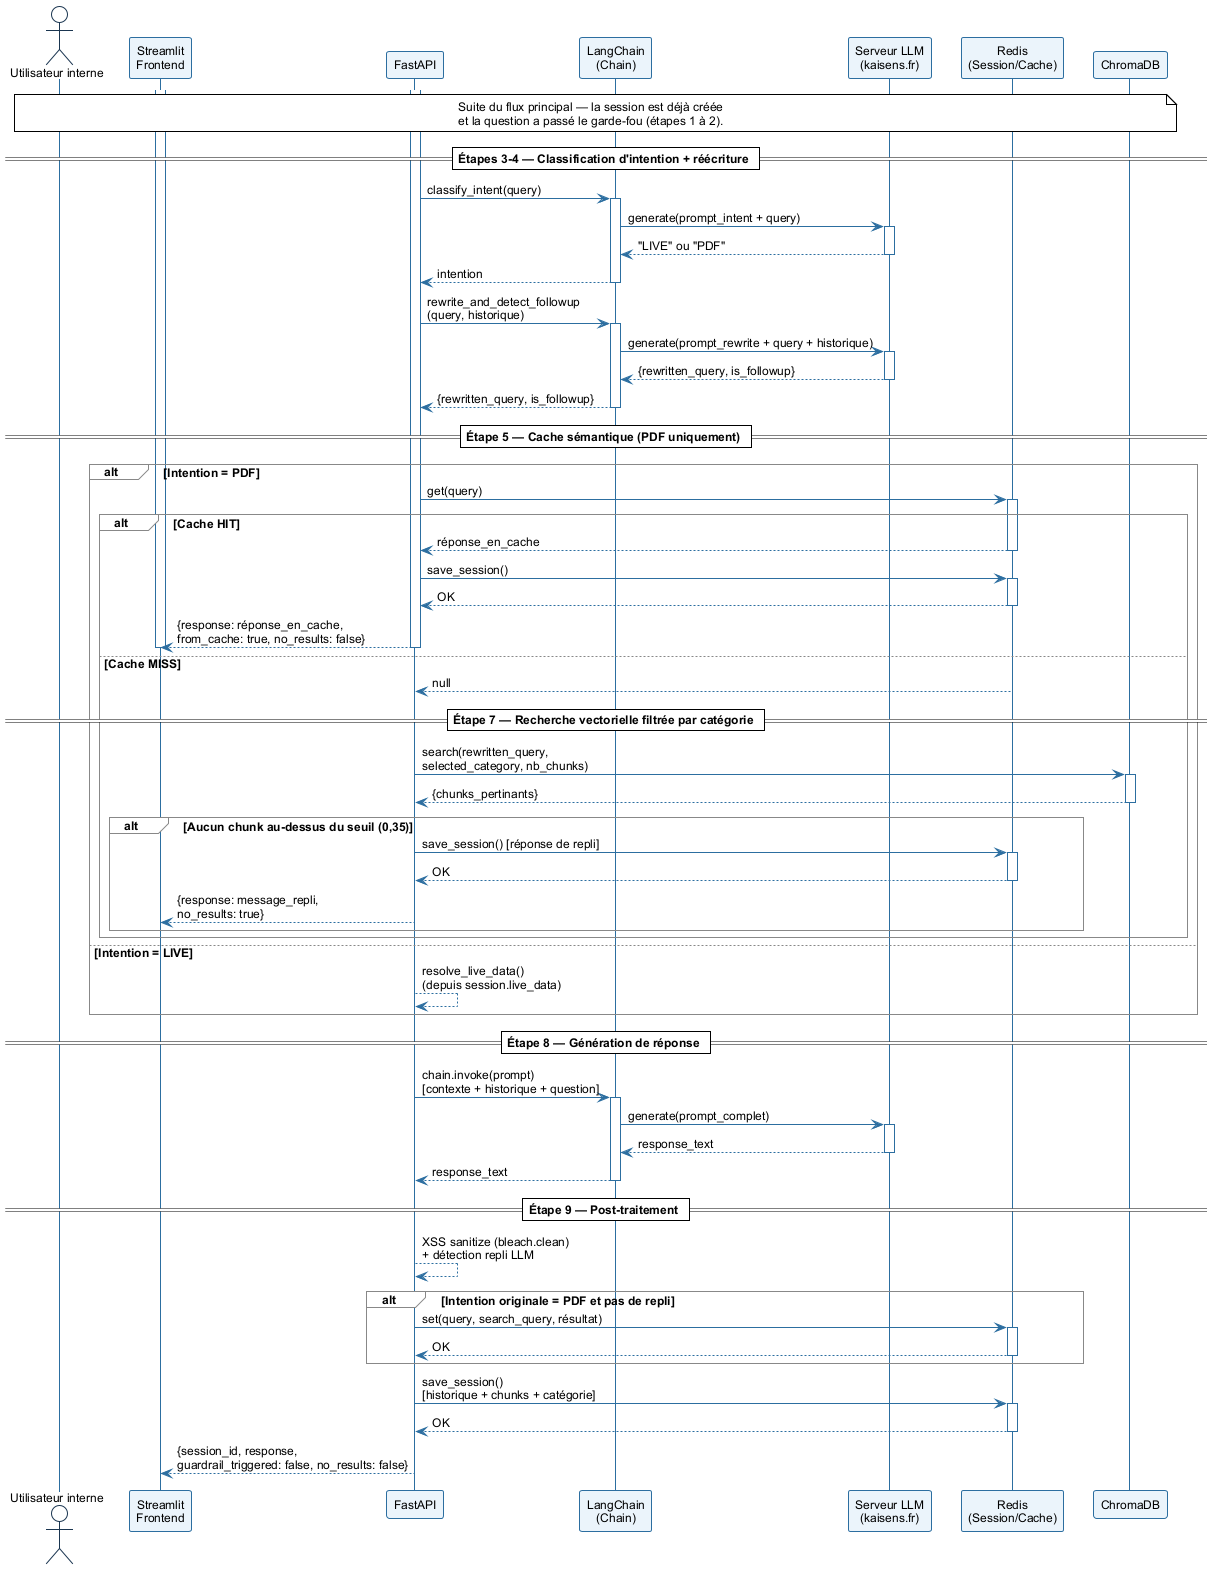
\includegraphics[width=1.15\textwidth]{diagramme/06_sequence_support.png}
\caption{Diagramme de séquences — Assistant technique (2/3) : pipeline RAG}
\label{fig:seq_support}
\end{figure}

La Figure~\ref{fig:seq_support_repli} illustre les flux de repli déclenchés
lorsqu'aucun document pertinent n'est trouvé dans ChromaDB (\texttt{no\_results=true}).
L'utilisateur dispose alors de deux options : prendre un rendez-vous ou signaler un bug.
Dans les deux cas, LangChain génère automatiquement une description à partir
de l'historique de conversation avant de soumettre la requête à l'API NetEthic.

\begin{figure}[H]
\centering
\hspace*{-0.1\textwidth}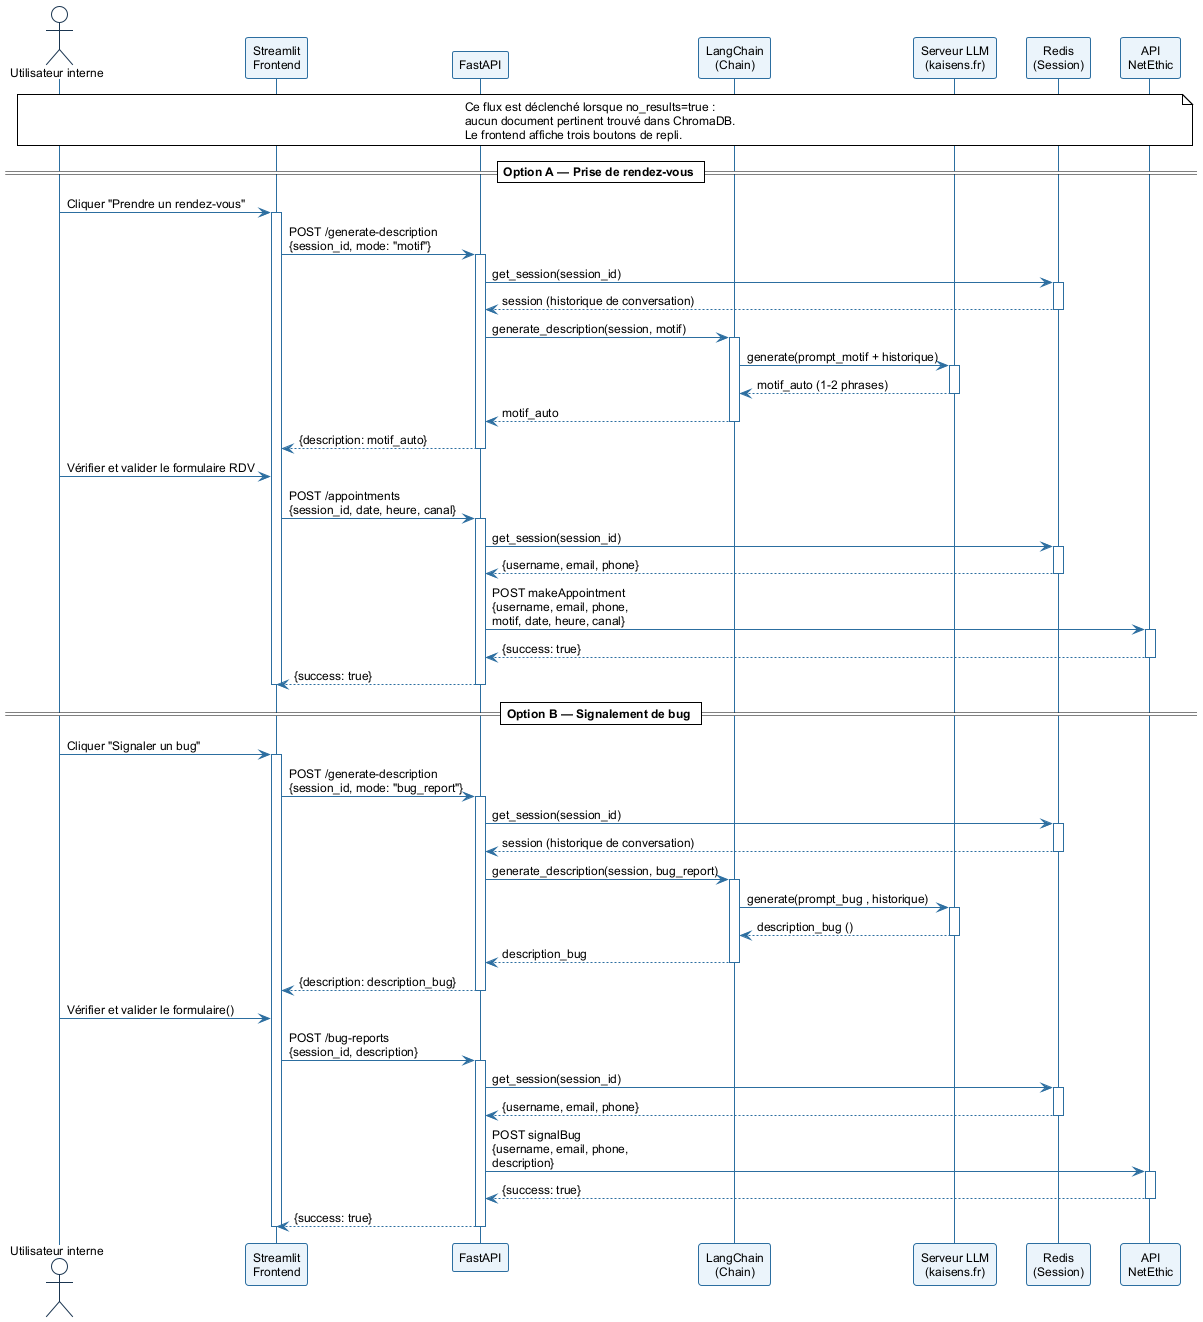
\includegraphics[width=1.15\textwidth]{diagramme/06b_sequence_support_repli.png}
\caption{Diagramme de séquences — Assistant technique (3/3) : flux de repli}
\label{fig:seq_support_repli}
\end{figure}

\subsection{Diagramme d'activité}

La Figure~\ref{fig:activite_support} représente le flux de traitement complet
d'un message par l'assistant technique, depuis la validation initiale
jusqu'à la génération de la réponse, en incluant les chemins de repli.

\begin{figure}[H]
\centering
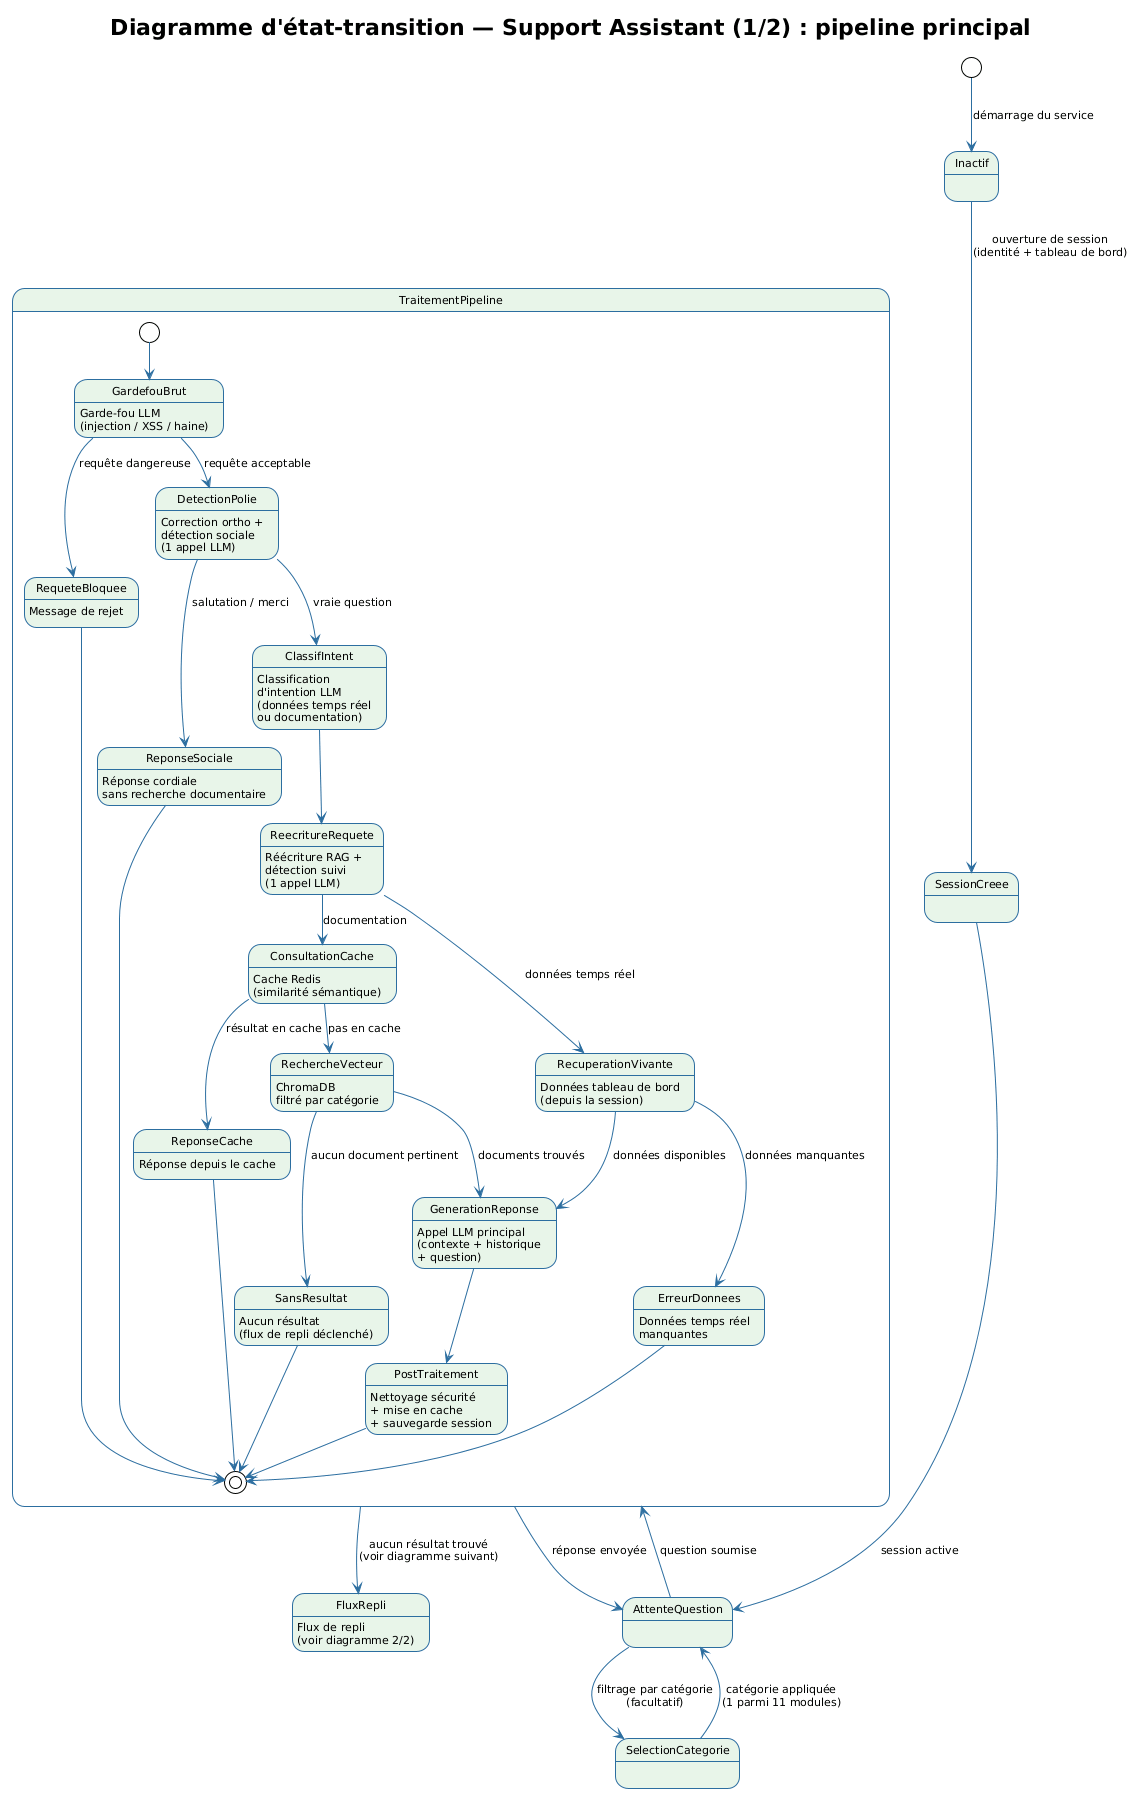
\includegraphics[width=0.95\textwidth]{diagramme/07a_etat_support_pipeline.png}
\caption{Diagramme d'activité — Assistant technique : pipeline et flux de repli}
\label{fig:activite_support}
\end{figure}

% ─────────────────────────────────────────────────────────────────────────────
\section{Module 3 — Assistant émotionnel}

\subsection{Conception générale}

L'assistant émotionnel est un assistant conversationnel dédié aux étudiants,
accessible via une interface Streamlit.
Il traite chaque message à travers un pipeline structuré reposant sur quatre mécanismes
complémentaires.

\textbf{Protection de l'échange.}
Chaque message passe par deux vérifications avant tout traitement :
une limitation du débit par fenêtre glissante Redis,
puis une analyse par un classifieur LLM à température nulle.
Les messages abusifs ou les tentatives de manipulation sont bloqués
à cette étape sans interrompre la session.

\textbf{Détection et réponse de crise.}
Si le classifieur identifie un signal de crise (idéation suicidaire ou intention de violence),
une réponse d'urgence est générée dans la langue de l'étudiant.
Les numéros d'aide sont ajoutés de façon systématique — jamais laissés à la discrétion du LLM.

\textbf{Mémoire persistante.}
Les informations partagées par l'étudiant (prénom, sources de stress, situation scolaire,
réussites) sont extraites automatiquement et stockées dans Redis avec une durée de vie
de trente jours. Ce profil enrichit le prompt système à chaque nouvelle session.

\textbf{Génération empathique.}
Pour les messages sûrs, l'assistant construit un prompt enrichi du profil mémorisé
et de l'historique de conversation, puis génère une réponse adaptée à la langue
et au contexte de l'étudiant, limitée à trois phrases.

\subsection{Diagramme de composants}

La Figure~\ref{fig:composants_emotionnel} illustre l'architecture en couches de l'assistant émotionnel et les interactions entre ses composants.

\begin{figure}[H]
\centering
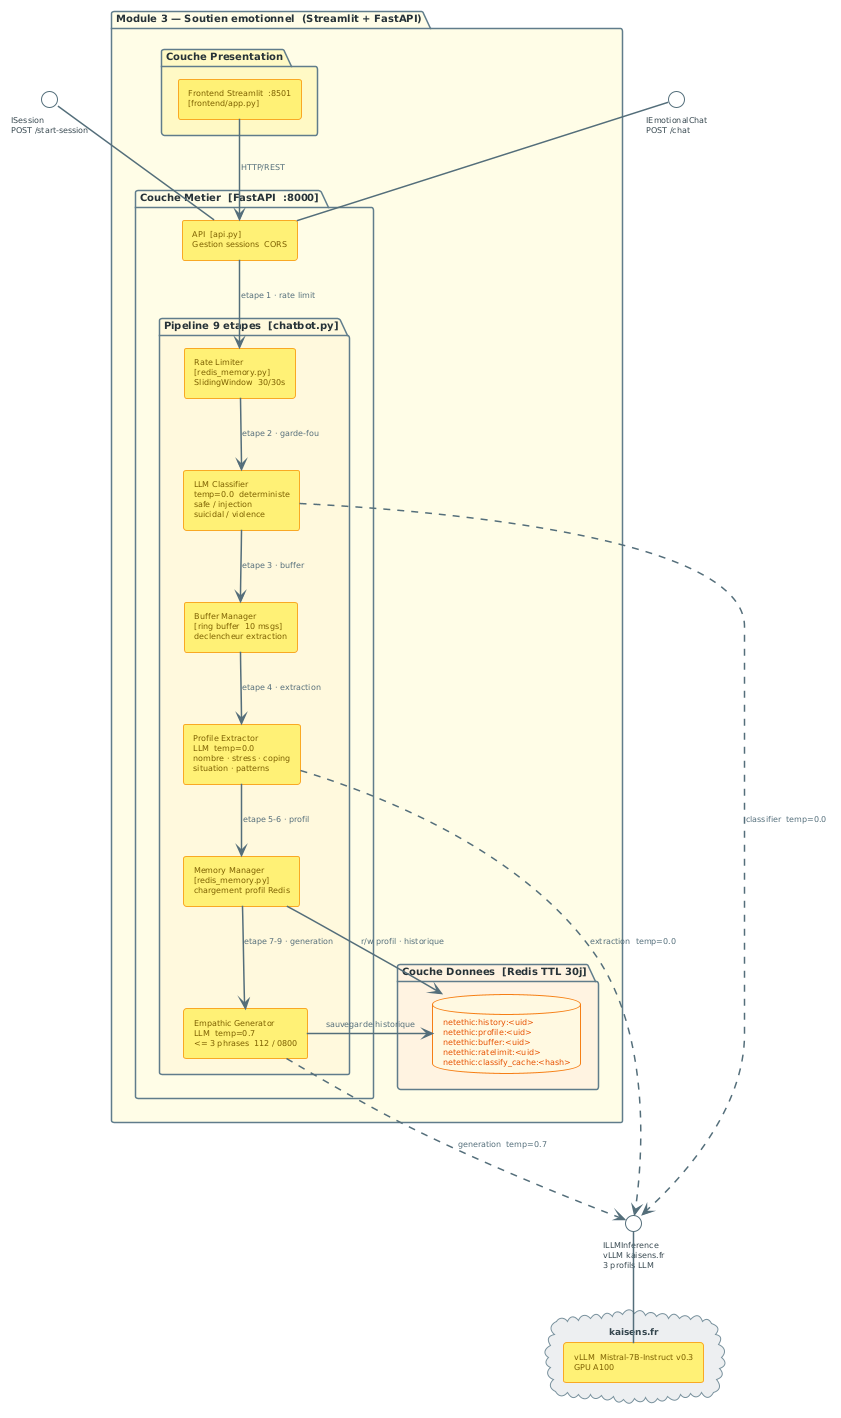
\includegraphics[width=\textwidth]{diagramme/20_composants_emotionnel.png}
\caption{Diagramme de composants — Assistant émotionnel}
\label{fig:composants_emotionnel}
\end{figure}

\subsection{Diagramme de déploiement}

La Figure~\ref{fig:deploiement_emotionnel} présente la stack Docker Compose de l'assistant émotionnel avec ses conteneurs et leurs interconnexions.

\begin{figure}[H]
\centering
\hspace*{-0.1\textwidth}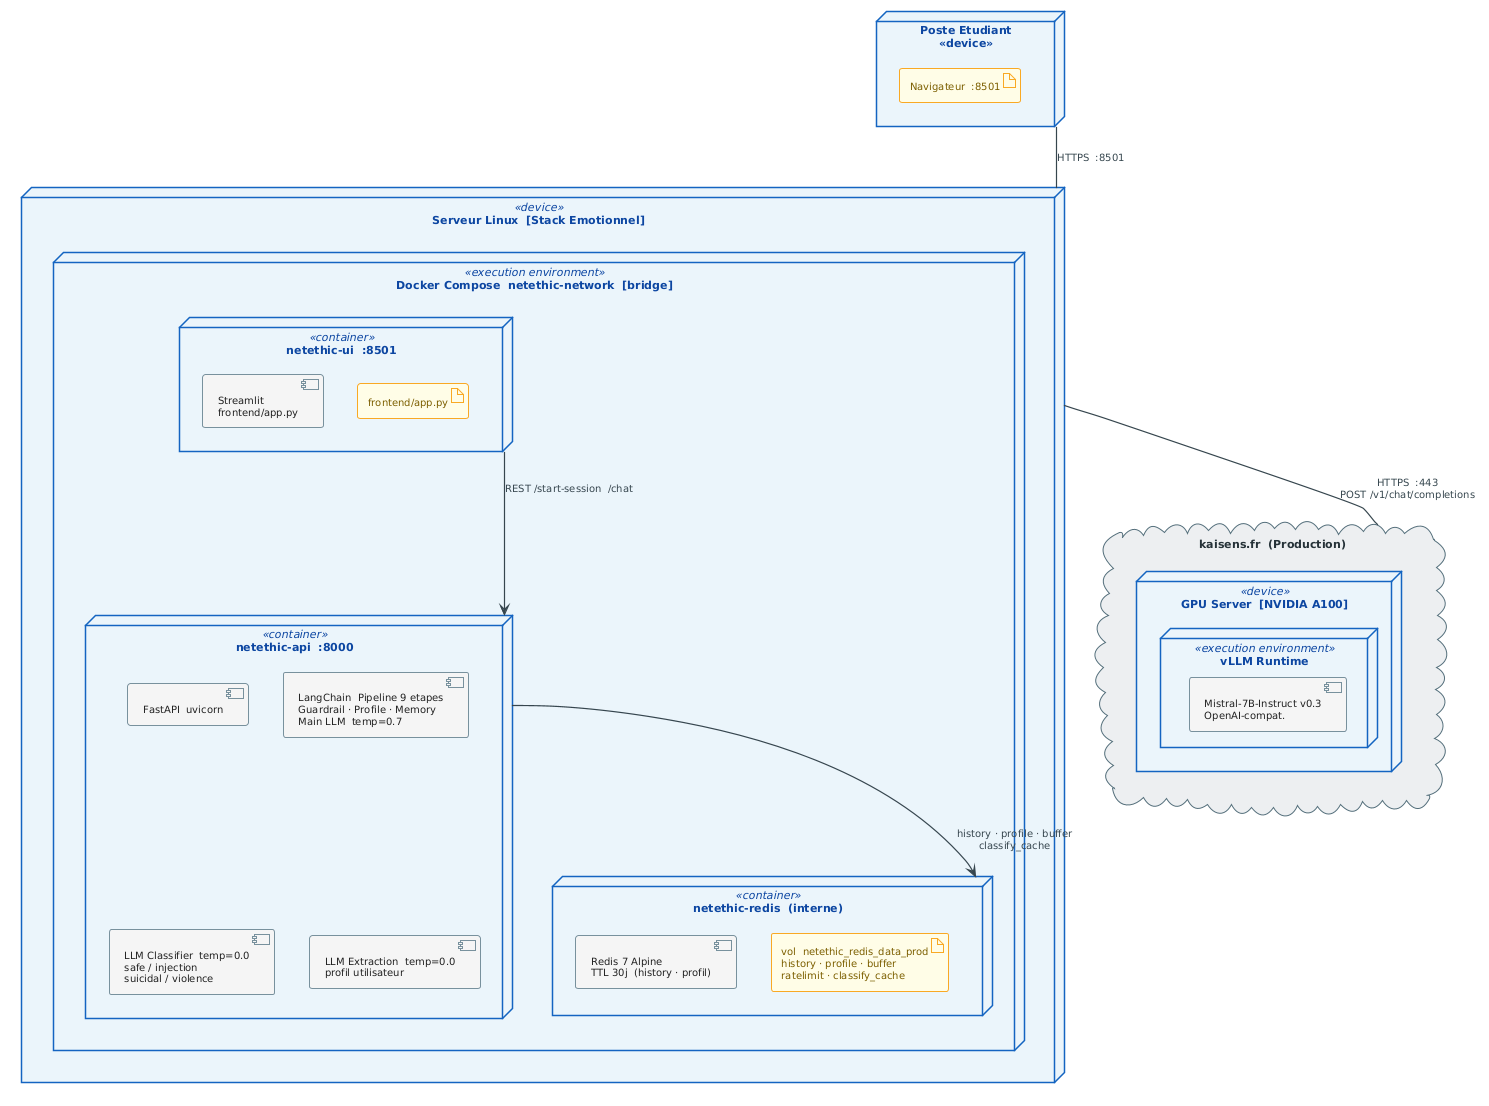
\includegraphics[width=1.2\textwidth]{diagramme/16_deploiement_emotionnel.png}
\caption{Diagramme de déploiement — Assistant émotionnel (stack Docker Compose)}
\label{fig:deploiement_emotionnel}
\end{figure}

\subsection{Diagramme de séquences}

La Figure~\ref{fig:seq_emotionnel_1} couvre les étapes 1 à 3 : validation de la session,
contrôle du débit et analyse par le garde-fou, avec ses quatre branches
(limite dépassée, contenu inapproprié, idéation suicidaire/violence, message sûr).

\begin{figure}[H]
\centering
\hspace*{-0.1\textwidth}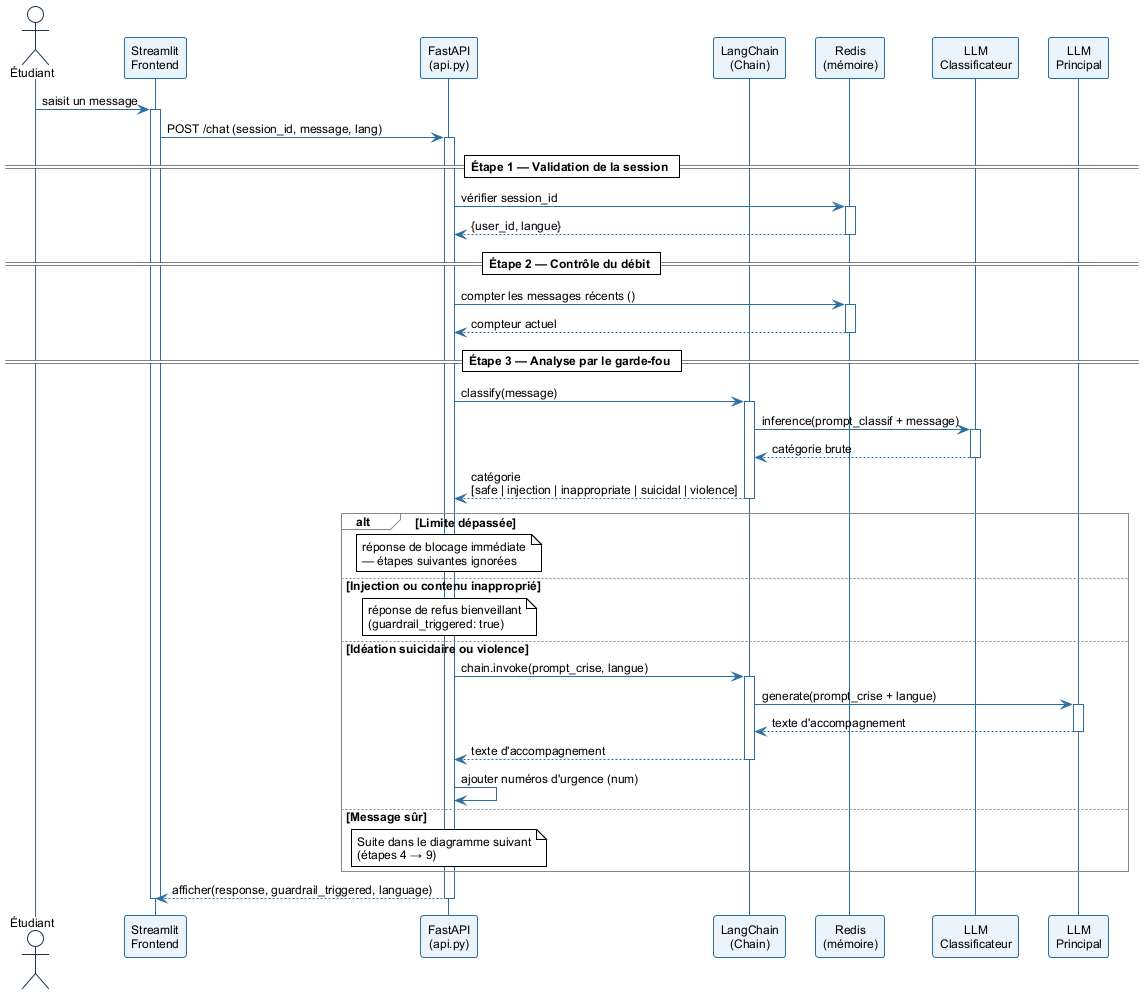
\includegraphics[width=1.15\textwidth]{diagramme/08b_sequence_emotionnel_1.png}
\caption{Diagramme de séquences — Assistant émotionnel (1/2) : validation et garde-fou}
\label{fig:seq_emotionnel_1}
\end{figure}

La Figure~\ref{fig:seq_emotionnel_2} détaille le chemin nominal (message sûr),
des étapes 4 à 9 : chargement du profil étudiant, enrichissement du prompt,
génération empathique par le LLM via LangChain, puis post-traitement et sauvegarde.

\begin{figure}[H]
\centering
\hspace*{-0.1\textwidth}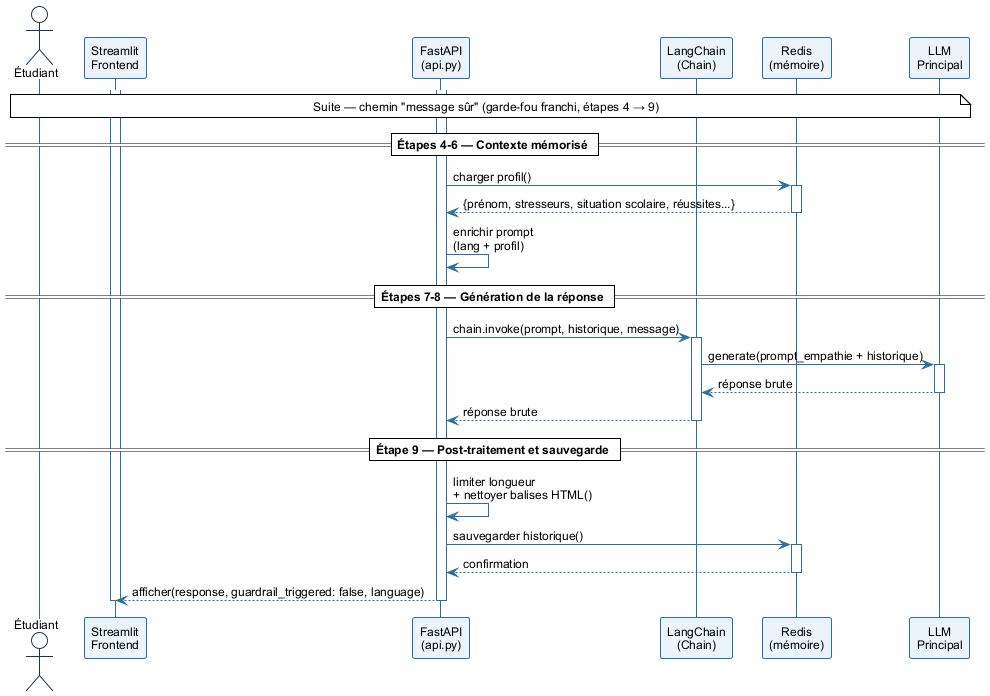
\includegraphics[width=1.15\textwidth]{diagramme/08b_sequence_emotionnel_2.png}
\caption{Diagramme de séquences — Assistant émotionnel (2/2) : génération et sauvegarde}
\label{fig:seq_emotionnel_2}
\end{figure}

\subsection{Diagramme d'activité}

La Figure~\ref{fig:activite_emo} représente le flux de traitement complet
d'un message par l'assistant émotionnel,
depuis la réception jusqu'à la journalisation de l'événement.

\begin{figure}[H]
\centering
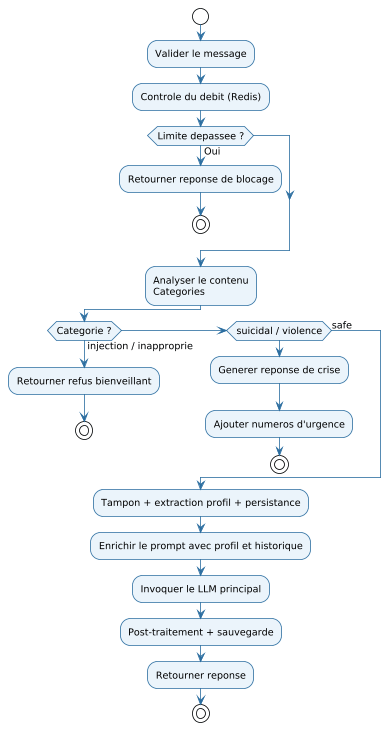
\includegraphics[width=0.6\textwidth]{diagramme/08_activite_emotionnel.png}
\caption{Diagramme d'activité — Assistant émotionnel}
\label{fig:activite_emo}
\end{figure}

% ─────────────────────────────────────────────────────────────────────────────
\section{Module 4 — Classificateur}

\subsection{Conception générale}

Le classificateur de harcèlement est un système d'analyse automatique des textes
soumis à la plateforme Netethic.
Sa conception repose sur la comparaison de quatre stratégies exécutées en parallèle,
permettant d'identifier la plus adaptée selon le type de texte et les conditions d'exécution.

\textbf{Modèle seul.}
Inférence directe du LLM sans contexte additionnel.
Approche généraliste et rapide, servant de référence de comparaison.

\textbf{Modèle avec ancrage juridique.}
Les passages de loi les plus pertinents sont récupérés depuis ChromaDB et injectés
dans la requête, ancrant la décision dans le droit français sur le harcèlement.

\textbf{Règles heuristiques.}
Correspondance par mots-clés spécifiques au français, sans recours au LLM.
Sert de mécanisme de repli rapide en cas d'indisponibilité du modèle.

\textbf{Hybride.}
Appel au LLM avec repli automatique sur les heuristiques en cas d'échec ou d'ambiguïté.
Cette stratégie combine la richesse sémantique du LLM et la robustesse des règles.

\subsection{Diagramme de composants}

La Figure~\ref{fig:composants_classificateur} illustre l'architecture interne du classificateur et la distribution des quatre stratégies de classification.

\begin{figure}[H]
\centering
\hspace*{-0.1\textwidth}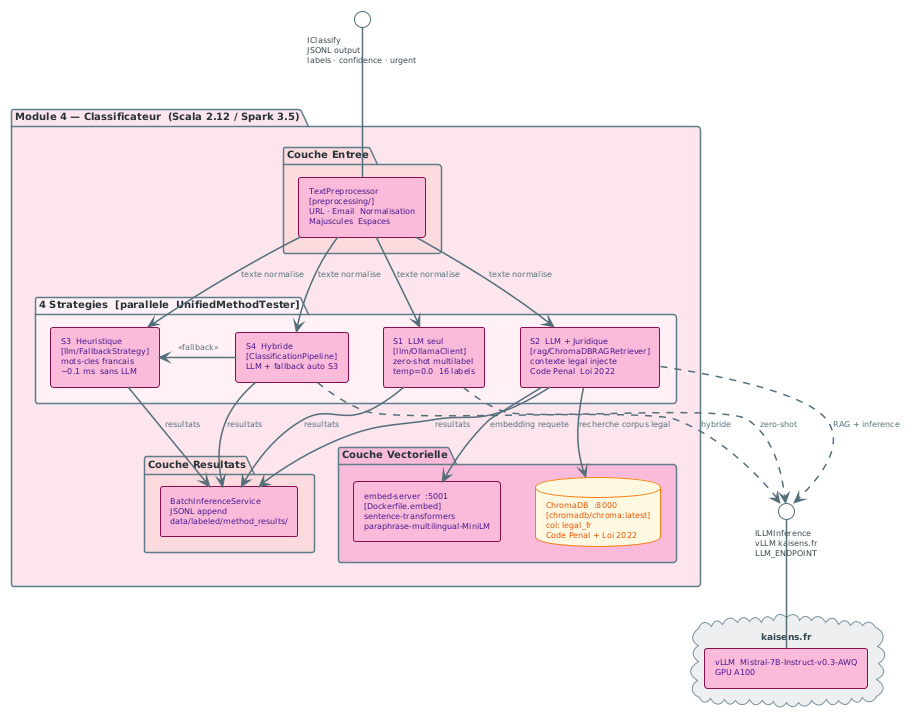
\includegraphics[width=1.2\textwidth]{diagramme/21_composants_classificateur.png}
\caption{Diagramme de composants — Classificateur de harcèlement}
\label{fig:composants_classificateur}
\end{figure}

\subsection{Diagramme de déploiement}

La Figure~\ref{fig:deploiement_classificateur} présente la stack Docker Compose du classificateur avec ses services et leurs interactions.

\begin{figure}[H]
\centering
\hspace*{-0.1\textwidth}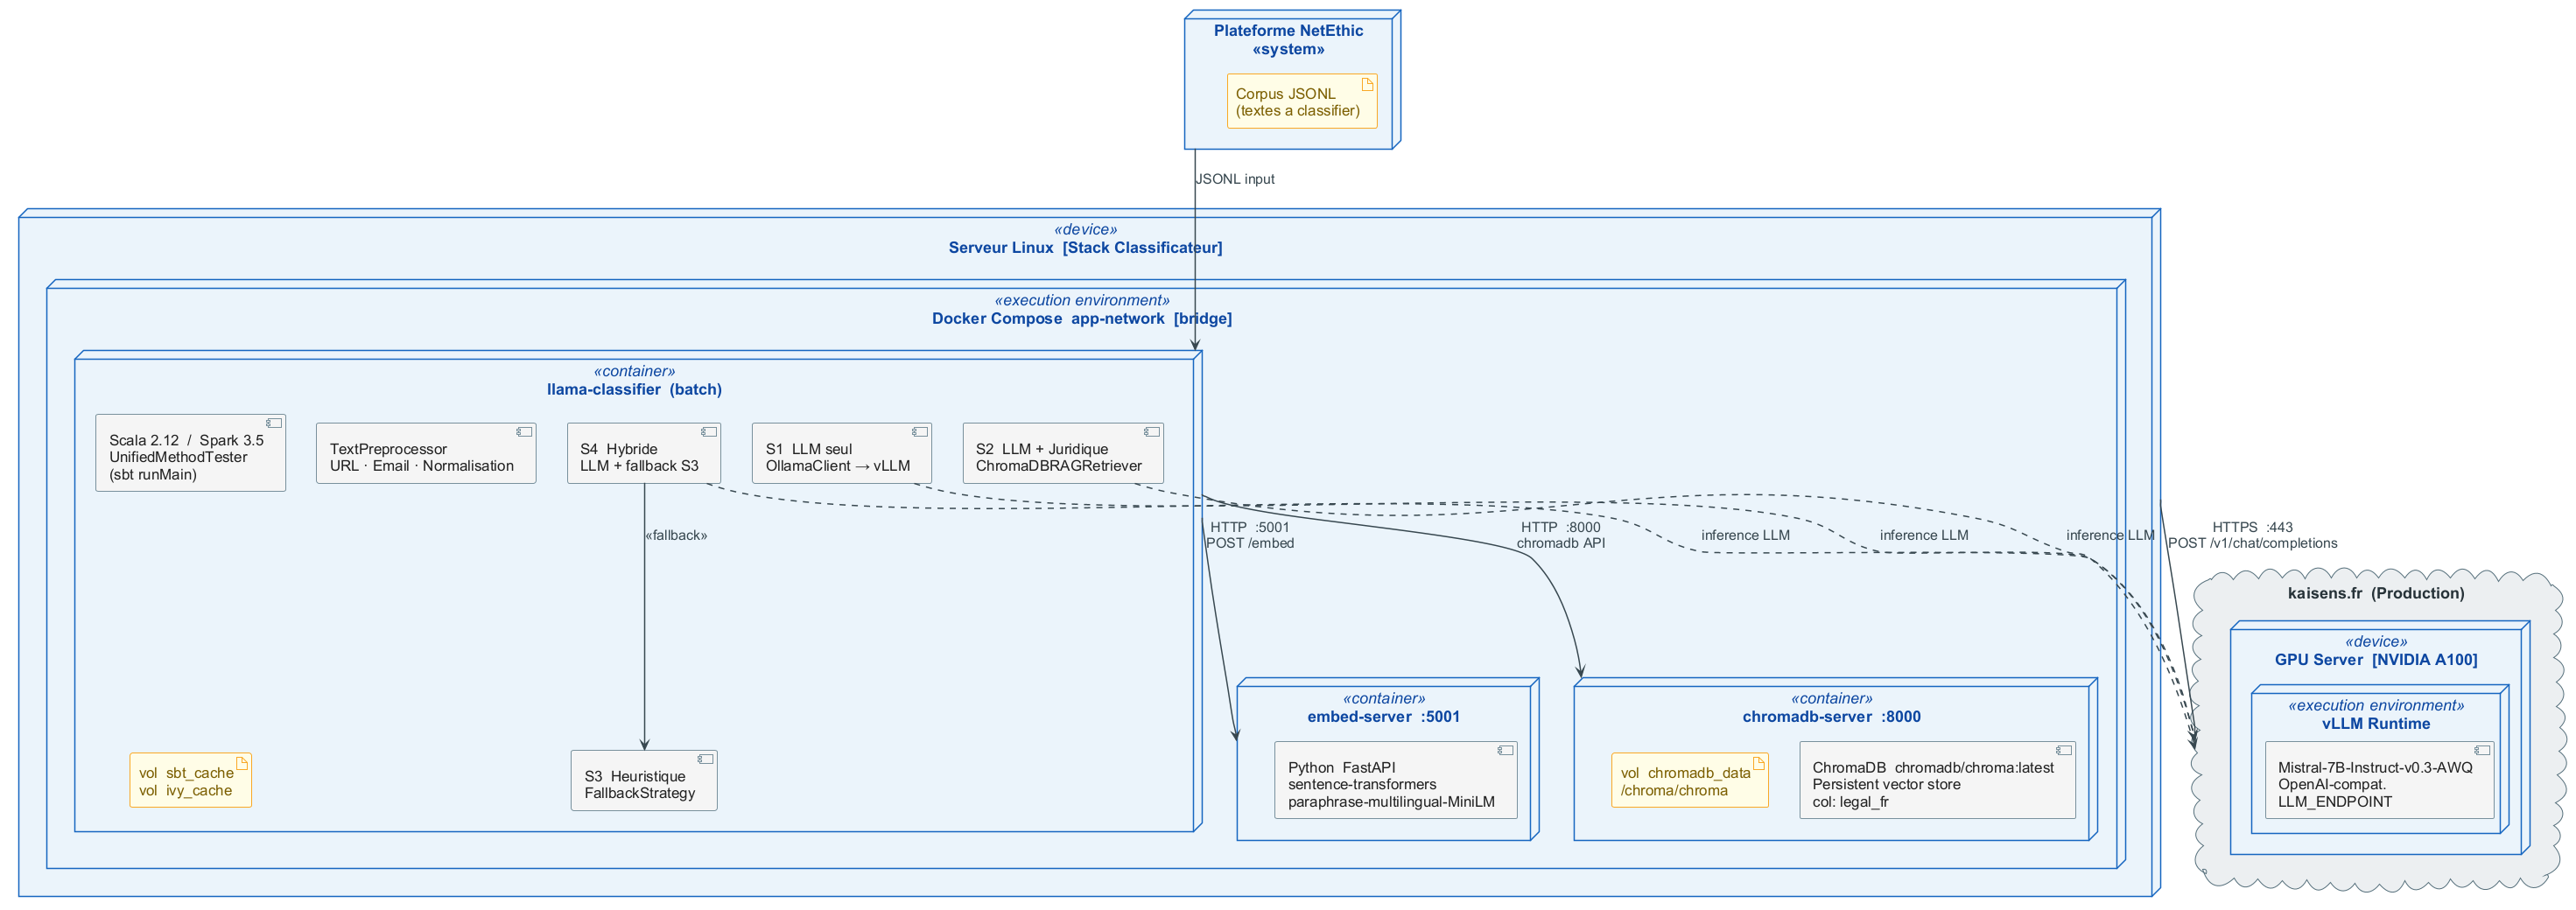
\includegraphics[width=1.2\textwidth]{diagramme/17_deploiement_classificateur.png}
\caption{Diagramme de déploiement — Classificateur de harcèlement (stack Docker Compose)}
\label{fig:deploiement_classificateur}
\end{figure}

\subsection{Diagramme de séquences}

La Figure~\ref{fig:seq_classif} illustre le flux de classification d'un texte.

\begin{figure}[H]
\centering
\hspace*{-0.1\textwidth}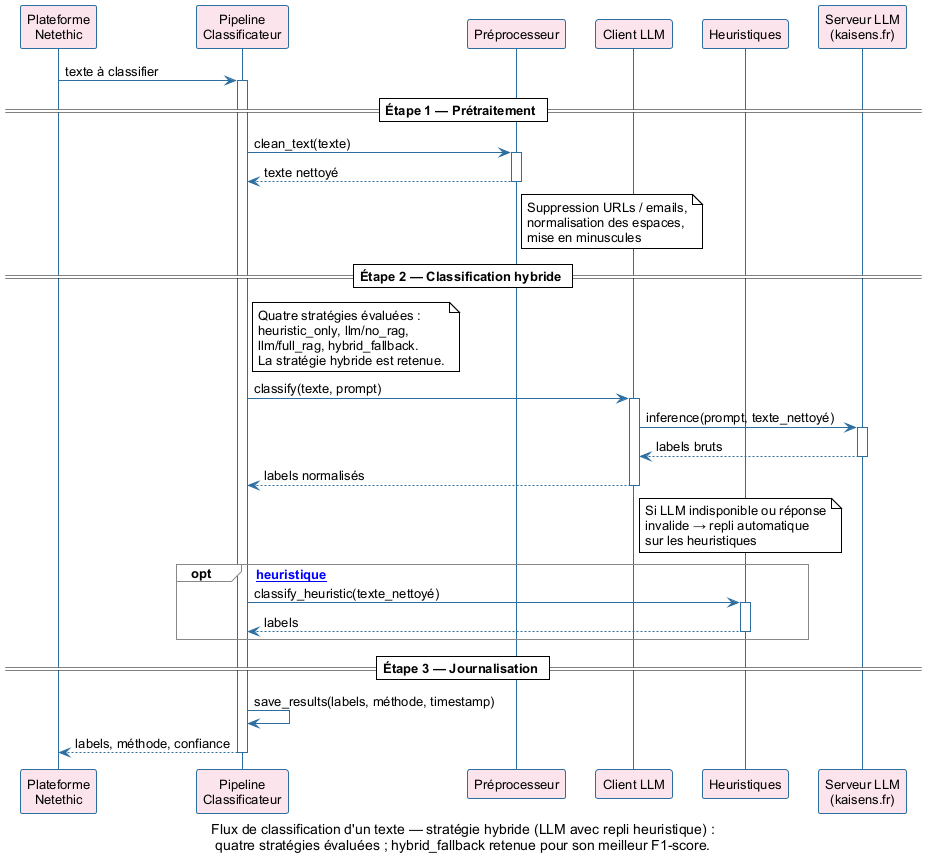
\includegraphics[width=1.2\textwidth]{diagramme/09_sequence_classificateur.png}
\caption{Diagramme de séquences — Classificateur de harcèlement}
\label{fig:seq_classif}
\end{figure}

\subsection{Diagramme d'activité}

La Figure~\ref{fig:activite_classif} représente le flux de traitement complet,
incluant les mécanismes de repli en cas d'échec.

\begin{figure}[H]
\centering
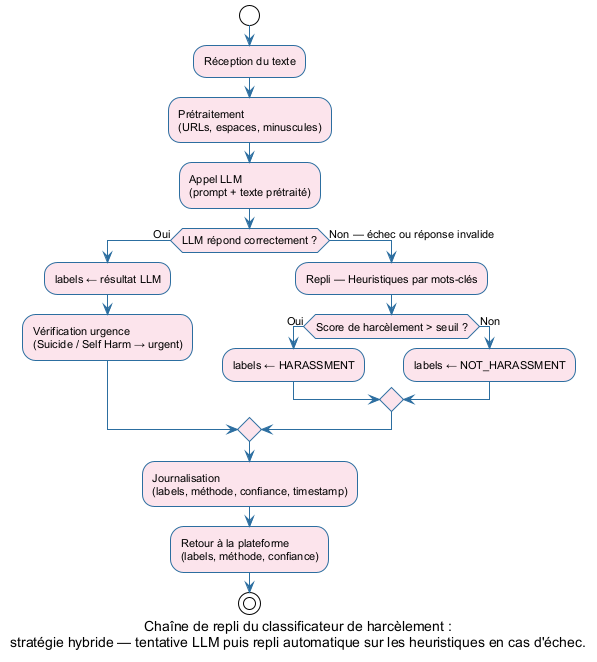
\includegraphics[width=0.95\textwidth]{diagramme/10_activite_classificateur.png}
\caption{Diagramme d'activité — Classificateur (chaîne de repli)}
\label{fig:activite_classif}
\end{figure}

% ─────────────────────────────────────────────────────────────────────────────
\section{Diagramme de classes (Application)}

Le diagramme de classes de la Figure~\ref{fig:classes_app} représente la structure statique
de l'application, c'est-à-dire les entités principales du système, leurs attributs et
les relations qui les unissent.

Les classes centrales sont les suivantes :

\begin{itemize}
    \item \textbf{ChatSession :} Représente une session conversationnelle.
          Attributs : \texttt{sessionId}, \texttt{userId}, \texttt{moduleType}, \texttt{createdAt}, \texttt{expiresAt}.
          Une session agrège plusieurs instances de \texttt{Message}.
    \item \textbf{Message :} Représente un message échangé au cours d'une session.
          Attributs : \texttt{messageId}, \texttt{content}, \texttt{role} (utilisateur/assistant), \texttt{timestamp}.
          Chaque message est associé à une \texttt{IntentClassification} et peut référencer un \texttt{Response}.
    \item \textbf{IntentClassification :} Encapsule le résultat de la classification d'intention.
          Attributs : \texttt{intent} (factual, chitchat, follow-up, forbidden), \texttt{confidence}.
    \item \textbf{DocumentChunk :} Représente un extrait de document indexé dans la base vectorielle.
          Attributs : \texttt{chunkId}, \texttt{content}, \texttt{embedding}, \texttt{category}, \texttt{sourceDocument}.
    \item \textbf{Response :} Encapsule la réponse générée par le LLM.
          Attributs : \texttt{responseId}, \texttt{content}, \texttt{sourceChunks}, \texttt{latency}, \texttt{cached}.
    \item \textbf{ReservationRequest :} Modélise une demande de réservation collectée par l'assistant Noa ou l'assistant technique.
          Attributs : \texttt{requestId}, \texttt{email}, \texttt{phone}, \texttt{requestedDate}, \texttt{channel}, \texttt{subject}.
    \item \textbf{HarassmentClassification :} Encapsule le résultat de l'analyse d'un texte par le classificateur.
          Attributs : \texttt{textId}, \texttt{labels}, \texttt{strategy}, \texttt{confidence}, \texttt{urgencyFlag}, \texttt{timestamp}.
    \item \textbf{EmotionalSignal :} Représente un signal de détresse détecté dans un message.
          Attributs : \texttt{signalType} (dépression, idéation suicidaire, solitude, anxiété, colère, addiction),
          \texttt{severity}, \texttt{detectedAt}.
\end{itemize}

\begin{figure}[H]
\centering
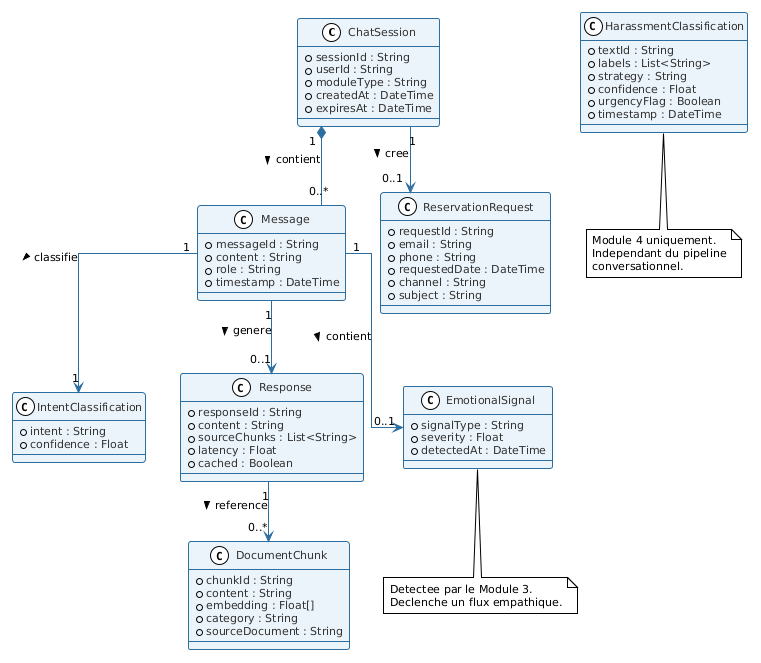
\includegraphics[width=0.95\textwidth]{diagramme/11_classes_application.png}
\caption{Diagramme de classes --- Architecture de l'application}
\label{fig:classes_app}
\end{figure}

% ─────────────────────────────────────────────────────────────────────────────
% PARTIE 2 — Mise en place du modèle d'IA générative
% ─────────────────────────────────────────────────────────────────────────────

\section{Préparation des bases de connaissances RAG}

Les modules assistant Noa et assistant technique reposent sur une architecture
\textit{Retrieval-Augmented Generation} (RAG) dont la qualité des réponses
dépend directement de la qualité et de la structure des documents indexés.
La phase de préparation consiste à transformer les sources documentaires brutes
en fichiers Markdown structurés et enrichis, exploitables par la base
vectorielle ChromaDB.

\subsection{Assistant Noa — sources documentaires publiques}

\paragraph{Extraction et conversion}\mbox{}\newline

La base de connaissances de Noa est constituée à partir du contenu du site public
de Netethic.
Les vingt-et-une pages du site ont été extraites et converties au format Markdown.
Cette conversion produit des fichiers textuels structurés,
plus adaptés au découpage en segments que les sources HTML brutes.

\paragraph{Enrichissement des fichiers Markdown}\mbox{}\newline

Après conversion, chaque fichier Markdown a été relu et enrichi
pour corriger les problèmes courants liés à l'extraction automatique~:

\begin{itemize}
    \item \textbf{Clarification des sous-titres :} Les intitulés de section trop courts
          ou ambigus ont été reformulés pour décrire explicitement le contenu
          de la rubrique et améliorer la précision de la recherche par similarité.
    \item \textbf{Complétion des informations manquantes :} Certains passages
          incomplets (tarifs, conditions d'accès, coordonnées) ont été complétés
          à partir des sources officielles.
    \item \textbf{Suppression des éléments non informatifs :} Les menus de navigation,
          pieds de page et formulaires ont été retirés pour ne conserver
          que le contenu textuel utile à la réponse.
\end{itemize}

\paragraph{Stratégie d'indexation parent-enfant}\mbox{}\newline

Les documents enrichis ont été découpés selon une stratégie parent-enfant~:
les segments courts (enfants) servent à la recherche par similarité sémantique,
tandis que les segments longs (parents) sont transmis au LLM pour générer
une réponse contextuellement riche.
Cette stratégie permet d'allier précision de la recherche et richesse
du contexte fourni au modèle de génération.

Le Tableau~\ref{tab:kb_noa} présente les statistiques de la base de connaissances
constituée pour Noa.

\vspace{6pt}
\begin{table}[H]
\centering
\caption{Statistiques de la base de connaissances — Assistant Noa}
\label{tab:kb_noa}
\begin{tabular}{|l|c|}
\hline
\textbf{Paramètre} & \textbf{Valeur} \\
\hline
Nombre de pages indexées    & 21 \\
\hline
Nombre de segments (chunks) & 177 \\
\hline
Modèle d'embedding          & \texttt{paraphrase-multilingual-mpnet-base-v2} \\
\hline
Seuil de pertinence         & 0,35 \\
\hline
Base vectorielle            & ChromaDB \\
\hline
\end{tabular}
\end{table}

\subsection{Assistant technique — documentation interne}

\paragraph{Sources documentaires}\mbox{}\newline

La base de connaissances de l'assistant technique est constituée à partir
de la documentation technique interne fournie par Smart-Conseil.
Elle couvre les onze catégories fonctionnelles de la plateforme Netethic~:
gestion des utilisateurs, paramétrage, tableaux de bord, rapports, notifications,
intégration, sécurité, conformité RGPD, support technique, administration
et facturation.

\paragraph{Transformation et structuration}\mbox{}\newline

Les documents fournis au format PDF ont été convertis au format Markdown.
Chaque fichier Markdown a ensuite été structuré par catégorie fonctionnelle,
en suivant le même processus d'enrichissement que pour la base de Noa~:
clarification des sous-titres, complétion des informations manquantes
et suppression des éléments non informatifs.

La collection ChromaDB de l'assistant technique est organisée en onze sous-collections,
une par catégorie fonctionnelle.
Cette organisation permet un filtrage précis lors de la recherche vectorielle~:
lorsqu'une catégorie est sélectionnée par l'utilisateur, la recherche
est restreinte aux documents de cette catégorie uniquement,
ce qui améliore la pertinence des résultats retournés.

% ─────────────────────────────────────────────────────────────────────────────
\section{Mise en place du classificateur de harcèlement}

Le classificateur de harcèlement est le module dont la mise en place
diffère fondamentalement des modules conversationnels~:
il ne repose pas sur un pipeline RAG mais sur un cycle complet
d'apprentissage automatique, depuis la collecte des données
jusqu'à l'évaluation comparative des stratégies de classification.

\subsection{Collecte des données}

Le corpus d'expérimentation est constitué de \textbf{977 textes multilingues}
(français et anglais), issus d'une application mobile de modération de contenu.
Tous les textes sont initialement étiquetés \textit{négatif} par l'application.
Le Tableau~\ref{tab:corpus_classif} décrit les caractéristiques du jeu de données brut.

\vspace{6pt}
\begin{table}[H]
\centering
\caption{Caractéristiques du corpus brut — Classificateur de harcèlement}
\label{tab:corpus_classif}
\small
\begin{tabular}{|l|l|}
\hline
\textbf{Caractéristique} & \textbf{Valeur} \\
\hline
Nombre de textes        & 977 \\
\hline
Langues                 & Français et anglais (mélangés) \\
\hline
Source                  & Application mobile de modération de contenu \\
\hline
Encodage                & Latin-1 (ISO-8859-1) \\
\hline
Étiquette initiale      & \textit{negative} (classification de l'application) \\
\hline
\end{tabular}
\end{table}

\subsection{Nettoyage et prétraitement}

L'analyse du corpus a révélé cinq catégories de bruits textuels~:
entités HTML (8 occurrences), images Markdown (3),
textes dépassant 128~caractères (152),
mentions d'utilisateurs (14) et URLs (5).

Un pipeline de prétraitement en cinq étapes a été développé pour normaliser
les textes avant inférence.
Le Tableau~\ref{tab:preprocessing_steps} décrit chaque étape.

\vspace{6pt}
\begin{table}[H]
\centering
\caption{Pipeline de prétraitement du corpus}
\label{tab:preprocessing_steps}
\small
\setlength{\tabcolsep}{4pt}
\begin{tabular}{|c|p{4cm}|p{8cm}|}
\hline
\textbf{Étape} & \textbf{Traitement} & \textbf{Description} \\
\hline
1 & Décodage HTML
  & Conversion des entités HTML (\texttt{\&amp;}, \texttt{\&\#39;}, etc.)
    en caractères lisibles. \\
\hline
2 & Suppression des balises
  & Élimination des balises HTML résiduelles (\texttt{<br>}, \texttt{<a href=...>}, etc.). \\
\hline
3 & Normalisation des mentions
  & Remplacement de toutes les mentions d'utilisateurs par un jeton générique. \\
\hline
4 & Normalisation des URLs
  & Remplacement de toutes les URLs par un jeton générique. \\
\hline
5 & Normalisation des espaces
  & Suppression des sauts de ligne multiples et collapsage des espaces superflus. \\
\hline
\end{tabular}
\end{table}

Le prétraitement conserve l'intégralité des 977~textes (aucune ligne vide
après nettoyage) et ne modifie que 2~prédictions sur 977 (0,2\,\%),
confirmant que les erreurs observées sont intrinsèques au modèle
et non aux données brutes.

\subsection{Augmentation des données}

Le corpus initial présente un déséquilibre de classes~:
après la phase de labeling (voir Section~\ref{subsec:labeling}),
647~textes sont confirmés dans la catégorie négative contre 330~textes
reclassifiés dans des catégories positives ou neutres.
Pour atténuer ce déséquilibre et améliorer la robustesse du modèle,
une stratégie d'augmentation des données a été appliquée à la classe minoritaire.

L'augmentation repose sur la paraphrase automatique par LLM~:
chaque texte de la classe minoritaire est soumis au modèle indépendant
avec une instruction de paraphrase, produisant une version reformulée
sémantiquement équivalente mais lexicalement différente.
Cette technique élargit la diversité des exemples d'entraînement
sans nécessiter de collecte de nouvelles données.

\subsection{Stratégie de labeling — LLM comme juge indépendant}
\label{subsec:labeling}

Pour évaluer la qualité des étiquettes produites par le modèle de classification
initial, une stratégie de \textit{LLM-as-a-Judge} a été adoptée~:
les 977~textes sont soumis à un modèle indépendant (\textbf{Groq API},
modèle \texttt{llama-3.1-8b-instant}) pour obtenir une annotation de référence.

Cette approche évite l'évaluation circulaire dans laquelle un modèle validerait
ses propres prédictions — biais qui rendrait les métriques sans valeur.

Le Tableau~\ref{tab:labeling_results} présente les résultats obtenus.

\vspace{6pt}
\begin{table}[H]
\centering
\caption{Résultats du labeling indépendant — LLM-as-a-Judge}
\label{tab:labeling_results}
\small
\begin{tabular}{|l|c|}
\hline
\textbf{Métrique} & \textbf{Valeur} \\
\hline
Textes confirmés dans la catégorie négative   & 647 / 977 \\
\hline
Textes reclassifiés (positif ou neutre)       & 330 / 977 \\
\hline
Précision du modèle initial                   & 66,2\,\% \\
\hline
Taux d'accord entre les deux modèles         & 63,4\,\% (619 / 977) \\
\hline
Impact du prétraitement sur les prédictions   & 0,2\,\% (2 / 977) \\
\hline
\end{tabular}
\end{table}

Les 33,8\,\% de désaccords s'expliquent principalement par un écart de domaine~:
le modèle initial a été entraîné sur des données formelles anglophones,
alors que le corpus contient de l'argot jeune francophone
(\og trop sous coter \fg{}, \og le meilleurrrrrr \fg{})
que ce modèle interprète incorrectement comme négatif.

\subsection{Entraînement et optimisation}

Quatre stratégies de classification ont été développées et comparées,
correspondant aux approches définies dans la partie conception de ce chapitre~:

\begin{enumerate}
    \item \textbf{Modèle seul :} Inférence directe du LLM sans contexte additionnel.
          Approche généraliste et rapide, servant de référence de comparaison.

    \item \textbf{Modèle avec ancrage juridique :} Les passages de loi les plus
          pertinents sont récupérés dynamiquement et injectés dans la requête,
          ancrant la décision dans le droit français sur le harcèlement.

    \item \textbf{Règles heuristiques :} Correspondance par mots-clés spécifiques
          au français, sans recours au LLM.
          Sert de mécanisme de repli rapide en cas d'indisponibilité du modèle.

    \item \textbf{Hybride :} Appel au LLM avec repli automatique sur les heuristiques
          en cas d'échec ou d'ambiguïté de la réponse du modèle.
\end{enumerate}

L'implémentation est disponible en deux versions complémentaires~:
\begin{itemize}
    \item \textbf{Version Python :} Adaptée aux expérimentations sur des corpus réduits,
          permettant de tester rapidement les quatre stratégies et de comparer
          leurs résultats avant mise en production.
    \item \textbf{Version Scala/Spark :} Conçue pour le traitement en parallèle
          à grande échelle avec Apache Spark~3.5, distribuant l'analyse sur
          l'ensemble des messages soumis à la plateforme Netethic.
\end{itemize}

\subsection{Évaluation des performances}
\label{subsec:eval_classif}

Le Tableau~\ref{tab:eval_classif} présente les métriques d'évaluation
des quatre stratégies sur le corpus de test.

\vspace{6pt}
\begin{table}[H]
\centering
\caption{Évaluation comparative des quatre stratégies de classification}
\label{tab:eval_classif}
\begin{tabular}{|l|c|c|c|}
\hline
\textbf{Stratégie} & \textbf{Précision} & \textbf{Rappel} & \textbf{F1-score} \\
\hline
Modèle seul                   & 0,295 & 0,437 & 0,352 \\
\hline
Modèle avec ancrage juridique & 0,223 & 0,606 & 0,326 \\
\hline
Règles heuristiques           & —     & —     & —     \\
\hline
Hybride                       & —     & —     & \textbf{0,619} \\
\hline
\end{tabular}
\end{table}

Le corpus de test comprend 1\,500~textes en français couvrant les 16~catégories
de la taxonomie (10~actes de harcèlement et 6~signaux de détresse).
La stratégie hybride atteint le meilleur F1-score global (0,619),
soit une amélioration de~76\,\% par rapport au modèle seul (0,352),
confirmant l'intérêt de combiner l'inférence LLM avec les règles heuristiques
comme mécanisme de repli.
La stratégie avec ancrage juridique améliore le rappel (0,606) au détriment
de la précision (0,223), ce qui traduit une tendance à surclasser les textes
ambigus comme relevant du harcèlement.

% ─────────────────────────────────────────────────────────────────────────────
\section*{Conclusion}

Ce chapitre a couvert la conception du système et la mise en place des modèles d'IA.
La partie conception a présenté l'architecture commune et les diagrammes UML de chaque module.
La mise en place a établi les bases de connaissances RAG (177~segments pour Noa,
11~collections pour l'assistant technique) et validé la stratégie hybride
pour le classificateur avec un F1-score de 0,619 sur 1\,500~textes de test.
Le chapitre suivant présente la réalisation concrète du système, les interfaces développées,
les résultats des tests automatisés et les évaluations de qualité.
